\documentclass{book} \usepackage{exsheets} \usepackage{xeCJK}
\usepackage{amsmath,amsfonts,amsthm,amssymb} \usepackage{bm}
\usepackage{hyperref} \usepackage{yhmath} \usepackage{caption}
\usepackage{pstricks-add} \usepackage{framed,mdframed}
\usepackage{graphicx,color} \usepackage{mathrsfs,xcolor}
\usepackage[all]{xy} \usepackage{fancybox}
\setcounter{MaxMatrixCols}{20}
\setCJKmainfont[BoldFont=SimHei]{SimSun} \SetupExSheets{
  counter-format = ch.se.qu , counter-within = section, solution/print
  = true }

\begin{document}
\chapter{线性方程组}
\section{向量空间和向量子空间}
\begin{question}
  为证明对向量空间,要求(i),(ii)是彼此独立的,请构造二维空间的两个子
  集:
  \begin{itemize}
  \item     对向量加法和减法都封闭,但对数乘不封闭.
  \item     对数乘封闭,但对向量加法不封闭.
  \end{itemize}
\end{question}
\begin{solution}
  \begin{itemize}
  \item     $\{(x,y):x,y\in \mathbf{Z}\}$.
  \item     $\{(a,0):a\in \mathbf{R}\}\cup \{(0,b):b\in \mathbf{R}\}$.
  \end{itemize}
\end{solution}
\begin{question}
  试判断$\mathbf{R}^3$的下列子集是否为子空间.
  \begin{itemize}
  \item     第一个分量$b_1=0$的向量平面.
  \item     $b_1=1$的向量$b$所成平面.
  \item     $b_1b_2=0$的向量$b$(这是平面$b_1=0$和平面$b_2=0$这两个子空间的
    并).
  \item     单个向量$b=(0,0,0)$.
  \item     向量$u=(1,1,0)$和$v=(2,0,1)$的所有组合.
  \item     满足$b_3-b_2+3b_1=0$的向量$(b_1,b_2,b_3)$
  \end{itemize}
\end{question}
\begin{solution}
  \begin{itemize}
  \item     是$\mathbf{R}^3$的子空间.
  \item     不是.因为对向量减法不封闭.
  \item     不是.对向量加法不封闭:$(0,1,2)+(1,0,2)=(1,1,4)$.
  \item     是.
  \item     是.
  \item     是.
  \end{itemize}
\end{solution}
\begin{question}
  验证$A$的化零空间是子空间,也即验证任何齐次方程组$Ax=0$的解$x$,对加法
  和数乘都封闭.举出一个$b\neq 0$时,$Ax=b$的解不是子空间的例子.
\end{question}
\begin{solution}
  对于任意$\lambda \in
  \mathbf{R}$,$A(\lambda x)=\lambda (Ax)=0$.且对于任意$Ax=0$的两个
  解$x_1,x_2$,
$$
A(\lambda_1x_1+\lambda_2
x_2)=\lambda_1(Ax_1)+\lambda_2(Ax_2)=0,\forall \lambda_1,\lambda_2\in
\mathbf{R}.
$$
因此矩阵$A$的化零空间是子空间.\\

当$b\neq
0$时,$Ax=b$的解必定不是子空间.这是因为$Ax=b$的任意两个解加起来,必定不
再是$Ax=b$的解,而是$Ax=2b$的解.(而且$Ax=2b$的解必定不是$Ax=b$的解).
\end{solution}
\section{$m\times n$方程组的解}
\begin{question}
  图2.2的阶梯矩阵是在一些可以作主元的元素为零(图中第3列和第5-8列就是)的
  情况下形成的.试画出主元都不为零情况下$5\times 9$矩阵的阶梯阵$U$.试举
  例证明,即使在$2\times 2$情况下,两个阶梯阵的和也可以不是阶梯阵,也即
  两个阶梯矩阵相加可以消去主元.
\end{question}
\begin{solution}
  $$ 
  \begin{pmatrix}
    *&*&*&*&*&*&*&*&*\\
    0&*&*&*&*&*&*&*&*\\
    0&0&*&*&*&*&*&*&*\\
    0&0&0&*&*&*&*&*&*\\
    0&0&0&0&*&*&*&*&*\\
  \end{pmatrix}
 $$
 两个阶梯矩阵相加未必是阶梯矩阵.举例如下:
$$
\begin{pmatrix}
  1&0&0&0\\
  0&0&1&0\\
  0&0&0&1\\
  0&0&0&0
\end{pmatrix}+
\begin{pmatrix}
  1&0&0&0\\
  0&0&-1&0\\
  0&0&0&1\\
  0&0&0&0
\end{pmatrix}=
\begin{pmatrix}
  2&0&0&0\\
  0&0&0&0\\
  0&0&0&2\\
  0&0&0&0
\end{pmatrix}
$$
两个相加的矩阵都是阶梯矩阵,加起来的结果却不是阶梯矩阵,因为加起来的矩阵
全是零的第二行在不全是零的第三行之上.二阶矩阵的例子如下:
$$
\begin{pmatrix}
  1&0\\
  0&1
\end{pmatrix}+
\begin{pmatrix}
  -1&0\\
  0&1
\end{pmatrix}=
\begin{pmatrix}
  0&0\\
  0&2
\end{pmatrix}
$$
加起来得到的矩阵第一行全是零,第二行不全是零,所以也不是阶梯矩阵.
\end{solution}
\begin{question}
  造一个未知数的个数多于方程的个数,但无解的最小方程组.
\end{question}
\begin{solution}
  \begin{align*}
    x+y+z&=1\\
    2x+2y+2z&=0
  \end{align*}
\end{solution}
\begin{question}
  求
$$
A=
\begin{pmatrix}
  1&2&0&1\\
  0&1&1&0\\
  1&2&0&1
\end{pmatrix}
$$
的分解式LU.决定基本变量和自由变量,求出$Ax=0$的通解,并将它写成类似
于(3)的形式.问$A$的秩是几?
\end{question}
\begin{solution}
 $$ 
 \begin{pmatrix}
   1&0&0\\
   0&1&0\\
   -1&0&1
 \end{pmatrix}
 \begin{pmatrix}
   1&2&0&1\\
   0&1&1&0\\
   1&2&0&1
 \end{pmatrix}=
 \begin{pmatrix}
   1&2&0&1\\
   0&1&1&0\\
   0&0&0&0
 \end{pmatrix}
 $$
 所以
$$
A=
\begin{pmatrix}
  1&0&0\\
  0&1&0\\
  1&0&1
\end{pmatrix}
\begin{pmatrix}
  1&2&0&1\\
  0&1&1&0\\
  0&0&0&0
\end{pmatrix}=LU.
$$
为了求出$Ax=0$的通解,设$x=
\begin{pmatrix}
  u\\
  v\\
  w\\
  y
\end{pmatrix}, $则$Ux=0$,即
$$
\begin{pmatrix}
  1&2&0&1\\
  0&1&1&0\\
  0&0&0&0
\end{pmatrix}
\begin{pmatrix}
  u\\
  v\\
  w\\
  y
\end{pmatrix}=
\begin{pmatrix}
  0\\
  0\\
  0\\
  0\\
\end{pmatrix}.
$$
基本变量为$u,v$,自由变量为$w,y$.由
$$
\begin{cases}
  u+2v+y=0\\
  v+w=0\\
\end{cases}
$$
解得
$$
\begin{cases}
  v=-w\\
  u=2w-y
\end{cases}.
$$
$$
x=
\begin{pmatrix}
  2w-y\\
  -w\\
  w\\
  y
\end{pmatrix}=w
\begin{pmatrix}
  2\\
  -1\\
  1\\
  0
\end{pmatrix}+y
\begin{pmatrix}
  -1\\
  0\\
  0\\
  1
\end{pmatrix}.
$$
矩阵$A$的秩是$2$,因为有两个基本变量.
\end{solution}
\begin{question}
  求矩阵
$$
A=
\begin{pmatrix}
  0&1&4&0\\
  0&2&8&0
\end{pmatrix}
$$
的阶梯阵$U$,基本变量,自由变量和$Ax=0$的通解.然后对$Ax=b$($b$的分量
为$b_1,b_2$)应用消去法,求出$Ax=b$相容(有解)的条件和(5)形式的通
解.又$A$的秩是几?
\end{question}
\begin{solution}
$$
\begin{pmatrix}
  1&0\\
  -2&1
\end{pmatrix}
\begin{pmatrix}
  0&1&4&0\\
  0&2&8&0
\end{pmatrix}=
\begin{pmatrix}
  0&1&4&0\\
  0&0&0&0
\end{pmatrix}.
$$
所以$A$的$U$矩阵为$
\begin{pmatrix}
  0&1&4&0\\
  0&0&0&0
\end{pmatrix}.  $ $Ax=0$,设$x=
\begin{pmatrix}
  u\\
  v\\
  w\\
  y
\end{pmatrix}, $基本变量是$v$,其它三个$u,w,y$都是自由变量.因此
$$
x=
\begin{pmatrix}
  u\\
  -4w\\
  w\\
  y
\end{pmatrix},
$$
可见,$Ax=0$的通解为
$$
u
\begin{pmatrix}
  1\\
  0\\
  0\\
  0
\end{pmatrix}+ w\begin{pmatrix}
  0\\
  -4\\
  1\\
  0
\end{pmatrix}+y
\begin{pmatrix}
  0\\
  0\\
  0\\
  1
\end{pmatrix}.
$$
$Ax=b$化为$Ux=L^{-1}b$.而
$$
L^{-1}b=
\begin{pmatrix}
  b_1\\
  -2b_1+b_2
\end{pmatrix}.
$$
所以$Ax=b$相容的条件为$-2b_{1}+b_{2}=0$.写成(5)形式的通解为
$$
u
\begin{pmatrix}
  1\\
  0\\
  0\\
  0
\end{pmatrix}+w
\begin{pmatrix}
  0\\
  -4\\
  1\\
  0
\end{pmatrix}+y
\begin{pmatrix}
  0\\
  0\\
  0\\
  1
\end{pmatrix}+
\begin{pmatrix}
  0\\
  b_1\\
  0\\
  0
\end{pmatrix}
$$矩阵$A$的秩是$1$.
\end{solution}
\begin{question}
  将矩阵换为前一题的转置矩阵
$$
A=
\begin{pmatrix}
  0&0\\
  1&2\\
  4&8\\
  0&0
\end{pmatrix}.
$$
将右端换为$b_1,b_2,b_3,b_4$,再做前一题.
\end{question}
\begin{solution}
  先将矩阵$A$化为U矩阵:
$$
\begin{pmatrix}
  1&0&0&0\\
  0&1&0&0\\
  -4&0&1&0\\
  0&0&0&1
\end{pmatrix}
\begin{pmatrix}
  0&1&0&0\\
  1&0&0&0\\
  0&0&1&0\\
  0&0&0&1
\end{pmatrix}
\begin{pmatrix}
  0&0\\
  1&2\\
  4&8\\
  0&0
\end{pmatrix}=
\begin{pmatrix}
  1&2\\
  0&0\\
  0&0\\
  0&0
\end{pmatrix}
$$
解方程$Ax=b$,即解方程$Ux=L^{-1}b$.设$x=
\begin{pmatrix}
  u\\
  v
\end{pmatrix}, $则
$$
Ux=
\begin{pmatrix}
  u+2v\\
  0\\
  0\\
  0
\end{pmatrix}=
\begin{pmatrix}
  b_2\\
  b_1\\
  -4b_{2}+b_3\\
  b_{4}
\end{pmatrix}.
$$
$Ax=b$有解当且仅当$b_4=0,-4b_2+b_3=0,b_1=0$.且$Ax=b$的解可以写成
$$
\begin{pmatrix}
  b_2-2v\\
  v
\end{pmatrix}
$$
的形式,或者
$$
v
\begin{pmatrix}
  -2\\
  1
\end{pmatrix}+
\begin{pmatrix}
  b_2\\
  0
\end{pmatrix}
$$
的形式.矩阵$A$的秩为$1$.
\end{solution}
\begin{question}
  求
$$
\begin{pmatrix}
  1&2&2\\
  2&4&5
\end{pmatrix}
\begin{pmatrix}
  u\\
  v\\
  w
\end{pmatrix}
$$
的通解,并照(5)那样把它写成$Ax=b$的特解与$Ax=0$的通解之和.
\end{question}
\begin{solution}
  将矩阵$A$化为阶梯阵,可得
$$
\begin{pmatrix}
  1&0\\
  -2&1
\end{pmatrix}
\begin{pmatrix}
  1&2&2\\
  2&4&5
\end{pmatrix}=
\begin{pmatrix}
  1&2&2\\
  0&0&1
\end{pmatrix}.
$$
解方程$Ax=b$,即解方
程$Ux=L^{-1}b$.设$x=(u,v,w)$,$b=(b_1,b_2)$.则$u$和$w$是基本变量,$v$是
自由变量.$Ux=L^{-1}b$即
$$
Ux=
\begin{pmatrix}
  u+2v+2w\\
  w
\end{pmatrix}=
\begin{pmatrix}
  b_1\\
  -2b_1+b_2
\end{pmatrix}.
$$
所以
\begin{align*}
  w&=-2b_1+b_2\\
  u&=b_1-2v-2w=b_1-2v-2(-2b_1+b_2)=-2v+5b_1-2b_2.
\end{align*}
所以题目中的方程的通解可以写成
$$
\begin{pmatrix}
  -2v+5b_1-2b_2\\
  v\\
  -2b_1+b_2
\end{pmatrix}=v
\begin{pmatrix}
  -2\\
  1\\
  0
\end{pmatrix}+
\begin{pmatrix}
  5b_1-2b_2\\
  0\\
  -2b_1+b_2
\end{pmatrix}
$$
的形式,其中$
\begin{pmatrix}
  5b_1-2b_2\\
  0\\
  -2b_1+b_2
\end{pmatrix}
$是$Ax=b$的一个特解.
\end{solution}
\begin{question}
  根据将第三个方程变为$0=0$(消去法完成之后)所加在$b$上的约束,写出
$$
\begin{pmatrix}
  1&0\\
  0&1\\
  2&3
\end{pmatrix}
\begin{pmatrix}
  u\\
  v
\end{pmatrix}=
\begin{pmatrix}
  b_1\\
  b_2\\
  b_3
\end{pmatrix}
$$
的有解右端$b$的集合.问秩是几?
\end{question}
\begin{solution}
  先将系数矩阵$A=
  \begin{pmatrix}
    1&0\\
    0&1\\
    2&3
  \end{pmatrix}
  $进行LU分解.
  \begin{align*}
    L^{-1}A=  \begin{pmatrix}
      1&0&0\\
      0&1&0\\
      0&-3&1
    \end{pmatrix}
            \begin{pmatrix}
              1&0&0\\
              0&1&0\\
              -2&0&1
            \end{pmatrix}
                    \begin{pmatrix}
                      1&0\\
                      0&1\\
                      2&3
                    \end{pmatrix}=
                         \begin{pmatrix}
                           1&0\\
                           0&1\\
                           0&0
                         \end{pmatrix}=U.
  \end{align*}
  方程$Ax=b$等价于$Ux=L^{-1}b$.设$x=
  \begin{pmatrix}
    u\\
    v\\
  \end{pmatrix},b=
  \begin{pmatrix}
    b_1\\
    b_2\\
    b_{3}
  \end{pmatrix}, $则$u,v$都是主变量.$Ux=L^{-1}b$可以写成
$$
\begin{pmatrix}
  u\\
  v\\
  0
\end{pmatrix}=
\begin{pmatrix}
  b_{1}\\
  b_{2}\\
  -3b_{2}-2b_{1}+b_{3}
\end{pmatrix}
$$
所以,有解右端$b$的集合是
$$
\left\{
  \begin{pmatrix}
    b_{1}\\
    b_{2}\\
    b_{3}
  \end{pmatrix}:-3b_{2}-2b_{1}+b_{3}=0.  \right\}
$$
矩阵的秩为$2$。
\end{solution}
\begin{question}
  求出$c$的值,使得下面的方程组有解
  \begin{align*}
    u+v+2w&=2\\
    2u+3v-w&=5\\
    3u+4v+w&=c
  \end{align*}
\end{question}
\begin{solution}
  该方程组可以改写成
$$
Ax=\begin{pmatrix}
  1&1&2\\
  2&3&-1\\
  3&4&1
\end{pmatrix}
\begin{pmatrix}
  u\\
  v\\
  w
\end{pmatrix}=
\begin{pmatrix}
  2\\
  5\\
  c
\end{pmatrix}=b.
$$
先将系数矩阵进行LU分解.
$$
L^{-1}A=\begin{pmatrix}
  1&0&0\\
  0&1&0\\
  0&-1&1
\end{pmatrix}
\begin{pmatrix}
  1&0&0\\
  0&1&0\\
  -3&0&1
\end{pmatrix}
\begin{pmatrix}
  1&0&0\\
  -2&1&0\\
  0&0&1
\end{pmatrix}
\begin{pmatrix}
  1&1&2\\
  2&3&-1\\
  3&4&1
\end{pmatrix}=
\begin{pmatrix}
  1&1&2\\
  0&1&-5\\
  0&0&0
\end{pmatrix}=U.
$$
方程$Ax=b$可以化为$Ux=L^{-1}b$,即
$$
\begin{pmatrix}
  1&1&2\\
  0&1&-5\\
  0&0&0
\end{pmatrix}
\begin{pmatrix}
  u\\
  v\\
  w
\end{pmatrix}=
\begin{pmatrix}
  2\\
  1\\
  c-7
\end{pmatrix}.
$$
解得$c=7$.
\end{solution}
\section{线性无关、基底和维数}
\begin{question}
  用求$c_1,c_2,c_3,c_4$的办法判定下列向量是否线性无关
$$
\mathbf{v}_1=
\begin{pmatrix}
  1\\
  1\\
  0\\
  0
\end{pmatrix},\mathbf{v}_2=
\begin{pmatrix}
  1\\
  0\\
  1\\
  0
\end{pmatrix},\mathbf{v}_3=
\begin{pmatrix}
  0\\
  0\\
  1\\
  1\\
\end{pmatrix},\mathbf{v}_4=
\begin{pmatrix}
  0\\
  1\\
  0\\
  1
\end{pmatrix}.
$$
\end{question}
\begin{solution}
  即判断线性方程组
 $$ 
 \begin{pmatrix}
   1&1&0&0\\
   1&0&0&1\\
   0&1&1&0\\
   0&0&1&1
 \end{pmatrix}
 \begin{pmatrix}
   c_1\\
   c_2\\
   c_3\\
   c_4
 \end{pmatrix}=
 \begin{pmatrix}
   0\\
   0\\
   0\\
   0
 \end{pmatrix}
 $$
 是否只有零解.为此通过行变换化系数矩阵为上阶梯矩阵.
 \begin{align*}
   &\begin{pmatrix}
     1&1&0&0\\
     1&0&0&1\\
     0&1&1&0\\
     0&0&1&1
   \end{pmatrix}\to
            \begin{pmatrix}
              1&1&0&0\\
              0&-1&0&1\\
              0&1&1&0\\
              0&0&1&1
            \end{pmatrix}\to
                     \begin{pmatrix}
                       1&1&0&0\\
                       0&-1&0&1\\
                       0&0&1&1\\
                       0&0&1&1
                     \end{pmatrix}\to
                              \begin{pmatrix}
                                1&1&0&0\\
                                0&-1&0&1\\
                                0&0&1&1\\
                                0&0&0&0
                              \end{pmatrix}
 \end{align*}
 所以上述向量线性相关.
\end{solution}
\begin{question}
  例5中$A$的列向量线性相关,问它的行向量是否也线性相关?
\end{question}
\begin{solution}
  线性无关.
\end{solution}
\begin{question}
  试证
$$
T=
\begin{pmatrix}
  a&b&c\\
  0&d&e\\
  0&0&f
\end{pmatrix}
$$
的对角元素有一个为零,它的行就线性相关.
\end{question}
\begin{solution}
  考虑逆否命题,也即证明,矩形$T$的三个行向量线性无关时,对角线元素全不
  为零.这在例4中已经证过.
\end{solution}
\begin{question}
  如果$\mathbf{v}_1,\mathbf{v}_2,\mathbf{v}_3$线性无
  关,问
  $\mathbf{w}_1=\mathbf{v}_1+\mathbf{v}_2$,$\mathbf{w}_2=\mathbf{v}_1+\mathbf{v}_3$,$\mathbf{w}_3=\mathbf{v}_2+\mathbf{v}_3$
  是否也线性无关?
\end{question}
\begin{solution}
  即判断使得方程
$$
a_1\mathbf{w}_1+a_2\mathbf{w}_2+a_3\mathbf{w}_3=\mathbf{0},
$$
成立的$(a_1,a_2,a_3)$是否只能是$(0,0,0)$.等价于判断线性方程组
$$
\begin{pmatrix}
  1&1&0\\
  1&0&1\\
  0&1&1
\end{pmatrix}
\begin{pmatrix}
  a_1\\
  a_2\\
  a_3
\end{pmatrix}=
\begin{pmatrix}
  0\\
  0\\
  0
\end{pmatrix}
$$
是否只有零解.为此,化系数矩阵为上阶梯矩阵.
$$
\begin{pmatrix}
  1&1&0\\
  1&0&1\\
  0&1&1
\end{pmatrix}\to
\begin{pmatrix}
  1&1&0\\
  0&-1&1\\
  0&1&1
\end{pmatrix}\to
\begin{pmatrix}
  1&1&0\\
  0&-1&1\\
  0&0&2
\end{pmatrix}.
$$
上阶梯矩阵线性满秩,因此$\mathbf{w}_1,\mathbf{w}_2,\mathbf{w}_3$线性无
关.
\end{solution}
\begin{question}
  用语言或在$x-y$平面上作图表示出$A=
  \begin{pmatrix}
    1&2\\
    3&6
  \end{pmatrix}
  $的列空间和行空间,并写出它们的基底.
\end{question}
\begin{solution}
  列空间:经过原点的直线$y=3x$.列空间的基底:$(1,3)$.\\
  行空间:经过原点的直线$y=2x$.行空间的基底:$(1,2)$.
\end{solution}
\begin{question}
  根据主元求出
$$
U=
\begin{pmatrix}
  0&1&4&3\\
  0&0&2&-2\\
  0&0&0&0\\
  0&0&0&0
\end{pmatrix}
$$
的列空间的基底.并将非基底列表示成基底列的线性组合.再求出$U$的行空间(它
是$\mathbf{R}^4$的另外一个子空间)的基底.
\end{question}
\begin{solution}
  列空间的基底是$
  \begin{pmatrix}
    1\\
    0\\
    0\\
    0\\
  \end{pmatrix},
  \begin{pmatrix}
    4\\
    2\\
    0\\
    0
  \end{pmatrix}.  $行空间的基底是$
  \begin{pmatrix}
    0&1&4&3
  \end{pmatrix},
  \begin{pmatrix}
    0&0&2&-2
  \end{pmatrix}.$
\end{solution}
\begin{question}
  假定我们把每一个$2\times 2$矩阵都看成一个“向量”.虽然它们并不是通常
  意义下的向量,但我们也有着矩阵加法和数乘矩阵的规则,而且二阶矩阵对这
  两种运算封闭.试求出该向量空间的一个基底.又问由所有阶梯阵$U$张成的子空
  间是什么样的?
\end{question}
\begin{solution}
  该向量空间的一个基底是
$$
\begin{pmatrix}
  1&0\\
  0&0
\end{pmatrix},
\begin{pmatrix}
  0&1\\
  0&0
\end{pmatrix},
\begin{pmatrix}
  0&0\\
  1&0
\end{pmatrix},
\begin{pmatrix}
  0&0\\
  0&1
\end{pmatrix}.
$$所有阶梯矩阵$U$张成的子空间是形如
$$
\begin{pmatrix}
  a&b\\
  0&c
\end{pmatrix}
$$
的矩阵的集合.
\end{solution}
\begin{question}
  $\mathbf{R}^3$中前两个分量相等的向量构成一个子空间.试求出该子空间的两
  个不同的基底.
\end{question}
\begin{solution}
  一个基底:$\{(0,1,0),(1,0,0)\}$.\\
  另一个基
  底
  :$\{(\frac{1}{2},\frac{\sqrt{3}}{2},0),(-\frac{\sqrt{3}}{2},\frac{1}{2},0)$.
\end{solution}
\begin{question}
  试举出下面这段话的一个反例:如果$\mathbf{v}_1,\cdots,\mathbf{v}_4$是
  向量空间$\mathbf{R}^4$的一个基底,又如果$W$是一个子空间,那
  么$\mathbf{v}_1,\cdots,\mathbf{v}_4$的某个子集构成$W$的基底.
\end{question}
\begin{solution}
  有人可能觉得$W=\{\mathbf{0}\}$,即零空间会是一个反例.但是这是不对的,
  因为零空间的基底是一个空集,而空集显然是
  $\{\mathbf{v}_1,\mathbf{v}_2,\mathbf{v}_3,\mathbf{v}_4\}$的子集.\\

  为了解决这个问题,我们先考虑一个相比之下更直观的问
  题:如果$\mathbf{v}_1,\mathbf{v}_2,\mathbf{v}_3$是$\mathbf{R}^3$的一个
  基底,尝试构造$\mathbf{R}^3$的一个子空间$W$,使
  得$\mathbf{v}_1,\mathbf{v}_2,\mathbf{v}_3$的任何子集都不是$W$的基底.之
  所以考虑这个问题是因为我们能在头脑中直接想象三维向量空
  间$\mathbf{R}^3$.事实上,
  令
  $\mathbf{u}_1=\mathbf{v}_1+\mathbf{v}_2$,$\mathbf{u}_2=\mathbf{v}_2+\mathbf{v}_3$.则
  向量$\mathbf{u}_1$和向量$\mathbf{u}_2$张成的二维子空
  间$W=\{\alpha\mathbf{u}_1+\beta\mathbf{u}_2:\alpha,\beta\in
  \mathbf{R}\}=\{\alpha\mathbf{v}_1+(\alpha+\beta)\mathbf{v}_2+\beta
  \mathbf{v}_3:\alpha,\beta\in \mathbf{R}\}$,它不能由
  $\mathbf{v}_1,\mathbf{v}_2,\mathbf{v}_3$的任何子集作为基底.\\

  有了这个例子,回到题目中的$\mathbf{R}^4$情形就好办了.我们要想办法构
  造$\mathbf{R}^4$的一个三维子空间,这个三维子空间中的一些向量要用
  到$\mathbf{v}_1,\mathbf{v}_2,\mathbf{v}_3,\mathbf{v}_4$这四个向量中的
  所有向量来进行线性表示.我们构造的例子是
$$
W=\{\alpha\mathbf{v}_1+\beta\mathbf{v}_2+\gamma\mathbf{v}_3+(\alpha+\beta+\gamma)\mathbf{v}_4:\alpha,\beta,\gamma\in\mathbf{R}\}.
$$
\end{solution}
\begin{question}
  假定$\mathbf{R}^3$中的向量$x,y,z$满足$x+y+z=0$.问$x,y,z$所张成的子空
  间的可能的维数是什么?对每一种可能举出一组$x,y,z$.
\end{question}
\begin{solution}
  \begin{itemize}
  \item     $0$维.$x=y=z=
    \begin{pmatrix}
      0\\
      0\\
      0
    \end{pmatrix}
    $.
  \item     $1$维.$x=
    \begin{pmatrix}
      1\\
      1\\
      1\\
    \end{pmatrix},y=
    \begin{pmatrix}
      2\\
      2\\
      2\\
    \end{pmatrix},z=
    \begin{pmatrix}
      -3\\
      -3\\
      -3\\
    \end{pmatrix}
    $.
  \item     $2$维.$x=
    \begin{pmatrix}
      1\\
      0\\
      0\\
    \end{pmatrix},y=
    \begin{pmatrix}
      0\\
      1\\
      0
    \end{pmatrix},z=
    \begin{pmatrix}
      -1\\
      -1\\
      0
    \end{pmatrix}.  $
  \item     不可能是三维.
  \end{itemize}
\end{solution}
\begin{question}
  $A=
  \begin{pmatrix}
    1&2&1\\
    0&0&4
  \end{pmatrix}.
  $试将$A$的行集合扩大为$\mathbf{R}^3$的基底,将$A$的列集合缩小
  为$\mathbf{R}^2$的基底.
\end{question}
\begin{solution}
  \begin{itemize}
  \item     扩大行集合为$\mathbf{R}^{3}$的基底:$
    \begin{pmatrix}
      1&2&1\\
      0&1&0\\
      0&0&4\\
    \end{pmatrix}.  $
  \item     缩小列集合为$\mathbf{R}^2$的基底:$
    \begin{pmatrix}
      1&1\\
      0&4
    \end{pmatrix}.  $
  \end{itemize}
\end{solution}
\begin{question}
  已知$V$的维数为$k$,试证(可用对偶定理2L)
  \begin{itemize}
  \item     $V$中任何$k$个无关向量都构成一个基底.
  \item     张成$V$的任何$k$个向量都构成一个基底.
  \end{itemize}
\end{question}
\begin{solution}
  \begin{itemize}
  \item     假如某$k$个线性无关的向量组不构成一个基底,意味着还存在向量无法
    用这$k$个向量进行线性表示.连同这个无法被线性表示的向量,可以得
    到$k+1$个线性无关的向量形成的向量组.这与$V$的维数是$k$矛盾($V$的维
    数是$K$意味着$V$的基,即$V$的极大线性无关组,中的向量个数为$k$).
  \item     由本题第一小步,只用证明张成$V$的$k$个向量线性无关.假如线性相关,
    则可以从中去掉一些向量,依旧张成$V$.这表明$V$的维数小于$k$,矛盾.
  \end{itemize}
\end{solution}
\begin{question}
  求$3\times 3$对称矩阵空间的维数和一个基底.
\end{question}
\begin{solution}
  $6$维.一个基底是
  \begin{align*}
    &
      \begin{pmatrix}
        1&0&0\\
        0&0&0\\
        0&0&0
      \end{pmatrix},
             \begin{pmatrix}
               0&0&0\\
               0&1&0\\
               0&0&0
             \end{pmatrix},
                    \begin{pmatrix}
                      0&0&0\\
                      0&0&0\\
                      0&0&1
                    \end{pmatrix}, \\&
                                       \begin{pmatrix}
                                         0&1&0\\
                                         1&0&0\\
                                         0&0&0
                                       \end{pmatrix},
                                              \begin{pmatrix}
                                                0&0&1\\
                                                0&0&0\\
                                                1&0&0
                                              \end{pmatrix},
                                                     \begin{pmatrix}
                                                       0&0&0\\
                                                       0&0&1\\
                                                       0&1&0
                                                     \end{pmatrix}.
  \end{align*}
\end{solution}
\begin{question}
  试证:如果$V$和$W$是$\mathbf{R}^5$的两个三维子空间,则$V$和$W$必定有
  共同的非零向量.
\end{question}
\begin{solution}
  设$V$的一组基底为$\mathbf{v}_1,\mathbf{v}_2,\mathbf{v}_3$.$W$的一组基
  底为$\mathbf{w}_1,\mathbf{w}_2,\mathbf{w}_{3}$.则由
  于$\mathbf{R}^{5}$是$5$维向量空间,因
  此
  $\mathbf{v}_1,\mathbf{v}_2,\mathbf{v}_{3},\mathbf{w}_1,\mathbf{w}_2,\mathbf{w}_{3}$
  必定线性相关,意即,必存在不全为零的
  数$a_{1},a_{2},a_{3},b_{1},b_{2},b_{3}$,使得
$$
a_{1}\mathbf{v}_{1}+a_{2}\mathbf{v}_{2}+a_{3}\mathbf{v}_{3}+b_{1}\mathbf{w}_{1}+b_{2}\mathbf{w}_{2}+b_{3}\mathbf{w}_{3}=\mathbf{0},
$$
即
$$
a_{1}\mathbf{v}_{1}+a_{2}\mathbf{v}_{2}+a_{3}\mathbf{v}_{3}=-b_{1}\mathbf{w}_{1}-b_{2}\mathbf{w}_{2}-b_{3}\mathbf{w}_{3}.
$$
可见,$V$和$W$有共同的非零向量.
\end{solution}
\section{四个基本子空间}
\begin{question}
  如果$m=n$,则$A$的化零空间等于左化零空间.问这一结论成立否?
\end{question}
\begin{solution}
  当$m=n$时,$A$是方阵.$A$的化零空间为$\{x:Ax=
  \begin{pmatrix}
    0\\
    0\\
    \vdots\\
    0
  \end{pmatrix}
  $,左化零空间为$\{x:x^{T}A=
  \begin{pmatrix}
    0&0&\cdots&0
  \end{pmatrix}.  $这两个空间显然是不一定相同的,除非$A$是对称矩阵.举例
  如下:令$A=
  \begin{pmatrix}
    1&1\\
    0&0
  \end{pmatrix}.
  $则$A$的化零空间为$\{(x,y):x+y=0,x,y\in \mathbf{R}\}$.$A$的左化零空间
  为$\{0\}$.
\end{solution}
\begin{question}
  试求出习题2.2.4中矩阵
$$
A=
\begin{pmatrix}
  0&1&4&0\\
  0&2&8&0
\end{pmatrix}
$$
的四种子空间的维数,并构造出它们的基底.
\end{question}
\begin{solution}
  先将矩阵$A$进行初等行变换化为上阶梯矩阵.
$$
\begin{pmatrix}
  0&1&4&0\\
  0&2&8&0
\end{pmatrix}\to
\begin{pmatrix}
  0&1&4&0\\
  0&0&0&0
\end{pmatrix}.
$$                                     
首先求$\mathcal{R}(A)$的基底和维数.$\mathcal{R}(A)$的基底是$
\begin{pmatrix}
  1\\
  0
\end{pmatrix},
$维数是$1$.\\

矩阵$A$的行空间的基底是$
\begin{pmatrix}
  1&4
\end{pmatrix},
$行空间的维数也是$1$.\\

矩阵$A$的零空间维数是$3$,零空间的一组基底是
$$
\begin{pmatrix}
  1\\
  0\\
  0\\
  0
\end{pmatrix},
\begin{pmatrix}
  0\\
  -4\\
  1\\
  0
\end{pmatrix},
\begin{pmatrix}
  0\\
  0\\
  0\\
  1
\end{pmatrix}.
$$

矩阵$A^T$的零空间的维数是$1$.零空间的基底是$
\begin{pmatrix}
  -2\\
  1
\end{pmatrix}.  $
\end{solution}
\begin{question}
  试求出下面矩阵的四种子空间的维数和基底
$$
A=
\begin{pmatrix}
  1&2&0&1\\
  0&1&1&0\\
  1&2&0&1
\end{pmatrix}.
$$
\end{question}
\begin{solution}
  先将矩阵$A$化为上阶梯型矩阵.
$$
\begin{pmatrix}
  1&2&0&1\\
  0&1&1&0\\
  1&2&0&1
\end{pmatrix}\to
\begin{pmatrix}
  1&2&0&1\\
  0&1&1&0\\
  0&0&0&0
\end{pmatrix}.
$$
可见,矩阵$A$的行空间的维数是$2$,行空间的一组基底为$
\begin{pmatrix}
  1&2&0&1\\
\end{pmatrix}
$和$
\begin{pmatrix}
  0&1&1&0
\end{pmatrix}
$.\\

矩阵$A$的列空间的维数也是$2$,列空间的一组基底为$
\begin{pmatrix}
  1\\
  0\\
  0
\end{pmatrix},
\begin{pmatrix}
  2\\
  1\\
  0
\end{pmatrix}.
$\\

矩阵$A$的化零空间的维数是$2$,化零空间的一组基底是$
\begin{pmatrix}
  0\\
  0\\
  1\\
  0
\end{pmatrix},
\begin{pmatrix}
  -1\\
  0\\
  0\\
  1
\end{pmatrix}.
$\\

矩阵$A^T$的化零空间的维数是$1$,矩阵$A^T$的化零空间的一组基底为$
\begin{pmatrix}
  0\\
  0\\
  1
\end{pmatrix}.$
\end{solution}
\begin{question}
  试描述下面矩阵的四种子空间
$$
A=
\begin{pmatrix}
  0&1&0&0\\
  0&0&1&0\\
  0&0&0&1\\
  0&0&0&0
\end{pmatrix}.
$$
\end{question}
\begin{solution}
  矩阵$A$的列空间是$3$维的,列空间的一组基底为$
  \begin{pmatrix}
    1\\
    0\\
    0\\
    0
  \end{pmatrix},
  \begin{pmatrix}
    0\\
    1\\
    0\\
    0
  \end{pmatrix},
  \begin{pmatrix}
    0\\
    0\\
    1\\
    0
  \end{pmatrix}.
  $\\
  矩阵$A$的行空间的维数也是$3$维.行空间的一组基底为$
  \begin{pmatrix}
    0&1&0&0
  \end{pmatrix},
  \begin{pmatrix}
    0&0&1&0
  \end{pmatrix},
  \begin{pmatrix}
    0&0&0&1
  \end{pmatrix}.
  $\\
  矩阵$A$的零空间的维数是$1$.零空间的一组基底为$
  \begin{pmatrix}
    1\\
    0\\
    0\\
    0
  \end{pmatrix}.
  $\\
  矩阵$A^T$的零空间的维数是$1$,$A^T$的零空间的一组基底为$
  \begin{pmatrix}
    1\\
    0\\
    0\\
    0
  \end{pmatrix}.  $
\end{solution}
\begin{question}
  试证:如果两个矩阵的积为零矩阵,$AB=0$,则$B$的列空间包含在$A$的化零空
  间之中.
\end{question}
\begin{solution}
  只用证明$B$的每一个列向量都属于$A$的化零空间即可.根据矩阵乘法定义这是
  显然的.
\end{solution}
\begin{question}
  试解释,为什么当且仅当$A$的秩等于$A'$的秩的时候$Ax=b$才可
  解,$A'$是把$b$加到$A$上所成的矩阵.
\end{question}
\begin{solution}
  首先注意到一点,矩阵$A$的行数和向量$b$的行数必定是相同的,因此才可以
  把
  向量$b$加到矩阵$A$上.\\

  当矩阵$A$的秩等于矩阵$A'$的秩的时候,表明添加的列向量$b$并不给矩
  阵$A$的列空间带来新的维数,意即向量$b$能被矩阵$A$的列向量线性表示,从
  而
  $Ax=b$有解.\\

  当$Ax=b$有解的时候,表明给矩阵$A$添加列向量$b$,并不给矩阵$A$的列空间
  带来新的维数.从而$A$与$A'$的秩相同.
\end{solution}
\begin{question}
  $a,b,c$已给,且$a\neq 0$.试求$d$,使
$$
A=
\begin{pmatrix}
  a&b\\
  c&d
\end{pmatrix}
$$
的秩为$1$.在求得的$d$之下,将$A$分解为$uv^T$.
\end{question}
\begin{solution}
  $d=\frac{bc}{a}$.
$$
A=
\begin{pmatrix}
  a\\
  c
\end{pmatrix}
\begin{pmatrix}
  1& \frac{b}{a}
\end{pmatrix}.
$$
\end{solution}
\begin{question}
  试求出秩为$1$矩阵
$$
A=
\begin{pmatrix}
  2&-2\\
  4&-4\\
  0&0
\end{pmatrix}\mbox{和}
\begin{pmatrix}
  1&1&2\\
  3&3&6
\end{pmatrix}
$$
的积$AB$.将$A$和$B$分别写成$uv^T$和$wz^T$,并验证积$AB$是$uz^T$的若干倍,
这倍数是内积$v^Tw$.
\end{question}
\begin{solution}
  $A=
  \begin{pmatrix}
    2\\
    4\\
    0
  \end{pmatrix}
  \begin{pmatrix}
    1&-1
  \end{pmatrix},B=
  \begin{pmatrix}
    1\\
    3\\
  \end{pmatrix}
  \begin{pmatrix}
    1&1&2
  \end{pmatrix}.  $
$$
AB=
\begin{pmatrix}
  2\\
  4\\
  0
\end{pmatrix}
\begin{pmatrix}
  1&-1
\end{pmatrix}
\begin{pmatrix}
  1\\
  3\\
\end{pmatrix}
\begin{pmatrix}
  1&1&2
\end{pmatrix}=-2
\begin{pmatrix}
  2\\
  4\\
  0
\end{pmatrix}
\begin{pmatrix}
  1&1&2
\end{pmatrix}.
$$
\end{solution}
\begin{question}
  在$x-y$平面上画出前题矩阵$A$的行空间和化零空间.
\end{question}
\begin{solution}
  画出来就免了.直接叙述吧.矩阵$A$的行空间形成直线$y=-x$.化零空间形成直
  线$y=x$.
\end{solution}
\begin{question}
  构造一个非线性函数$y(x)$,是一对一的,但不是映上的;再构造一个非线性函
  数,是映上的,但不是一对一的.
\end{question}
\begin{solution}
  $y=\frac{1}{x}$;$y=\tan x$.
\end{solution}
\begin{question}
  当且仅当对$A^T$唯一性成立时,对$A$存在性才成立.反之亦然.试解释,这是
  为什么?
\end{question}
\begin{solution}
  当方程组$A^Tx=b$有唯一解或无解时,表明矩阵$A^T$列满秩,即矩阵$A$行满
  秩.所以方程组$Ax=c$存在解.\\

反之,当方程组$Ax=c$存在解时,意味着矩阵$A$行满秩,即矩阵$A^T$列满秩,所
以$A^Tx=b$有唯一解或无解.
\end{solution}
\begin{question}
  $A=
  \begin{pmatrix}
    1&1&0
  \end{pmatrix}
$试构造$A$和$A^T$的所有可能的左逆或右逆矩阵.
\end{question}
\begin{solution}
 矩阵$A$的秩为$1$,是行满秩矩阵.所以矩阵有右逆.设矩阵$A$的右逆矩阵为$
 \begin{pmatrix}
   x\\
y\\
z
 \end{pmatrix},
$则
$$
\begin{pmatrix}
  1&1&0
\end{pmatrix}
\begin{pmatrix}
  x\\
y\\
z
\end{pmatrix}=
\begin{pmatrix}
  1
\end{pmatrix}.
$$
基本变量是$x$,自由变量是$y$和$z$.所以所有可能的右逆矩阵为$
\begin{pmatrix}
  1-y\\
y\\
z
\end{pmatrix}.
$

\end{solution}
\section{正交向量和正交子空间}
\begin{question}
  求$x=
  \begin{pmatrix}
    1\\
    4\\
    0\\
    2
  \end{pmatrix}
  $,$y=
  \begin{pmatrix}
    2\\
    -2\\
    1\\
    3
  \end{pmatrix}
  $的长度和内积.
\end{question}
\begin{solution}
  $||x||=\sqrt{x^Tx}=\sqrt{1^2+4^2+0^2+2^2}=\sqrt{21}$.$||y||=\sqrt{y^Ty}=\sqrt{2^2+(-2)^2+1^2+3^2}=3
  \sqrt{2}$.
$$
x^Ty=1\cdot 2+4\cdot (-2)+0\cdot 1+2\cdot 3=0.
$$
\end{solution}
\begin{question}
  试在$\mathbf{R}^2$中先举出一组线性无关但彼此不正交的向量,从而就证明
  了上述定理的逆定理不成立.再举出一组彼此正交但不是线性无关的向量,从而
  说明定理中非零这一条件不可去.
\end{question}
\begin{solution}
  \begin{itemize}
  \item   $(2,2),(1,2)$.
  \item   $(0,0),(1,1)$.
  \end{itemize}
\end{solution}
\begin{question}
  解析几何告诉我们,平面上两条直线,如果互相垂直,则斜率的乘积为$-1$.试
  将这一点应用于向量$x=(x_1,x_2)$和$y=(y_1,y_2)$,它们的斜率
  为$\frac{x_2}{x_1}$和$\frac{y_2}{y_1}$,从而再一次导出正交的条
  件$x^Ty=0$.
\end{question}
\begin{solution}
  $$
  \frac{x_2}{x_1}\cdot \frac{y_2}{y_1}=-1\Rightarrow
  x_1y_1+x_2y_2=0\Rightarrow x^Ty=0.
  $$
\end{solution}
\begin{question}
  试证,$i\neq j$时$B$的第$i$行正交于$B^{-1}$的第$j$列.
\end{question}
\begin{solution}
  因为$BB^{-1}=I$,当$i\neq
  j$时,矩阵$I$的第$i$行第$j$列元素为$0$,而这个元素恰好就是矩
  阵$B$的第$i$行向量与矩阵$B^{-1}$的第$j$列向量内积的结果.
\end{solution}
\begin{question}
  指出下列向量中正交的对
$$
v_1=
\begin{pmatrix}
  1\\
  2\\
  -2\\
  1
\end{pmatrix},v_{2}=
\begin{pmatrix}
  4\\
  0\\
  4\\
  0\\
\end{pmatrix},v_3=
\begin{pmatrix}
  1\\
  -1\\
  -1\\
  -1
\end{pmatrix}.
$$
\end{question}
\begin{solution}
  $v_1$和$v_3$正交,$v_2$和$v_3$也正交.
\end{solution}
\begin{question}
  试求出$\mathbf{R}^3$中与$(1,1,1)$和$(1,-1,0)$都正交的所有向量.并用已
  知的两个向量与求得的一个向量构成$\mathbf{R}^3$的一个彼此正交的单位向
  量组.
\end{question}
\begin{solution}
  设与$(1,1,1)$和$(1,-1,0)$都正交的向量为$(x,y,z)$.则
$$
\begin{pmatrix}
  1&1&1\\
  1&-1&0
\end{pmatrix}
\begin{pmatrix}
  x\\
  y\\
  z
\end{pmatrix}=
\begin{pmatrix}
  0\\
  0
\end{pmatrix}.
$$
即
$$
\begin{pmatrix}
  1&1&1\\
  0&-2&-1
\end{pmatrix}
\begin{pmatrix}
  x\\
  y\\
  z
\end{pmatrix}=
\begin{pmatrix}
  0\\
  0
\end{pmatrix}.
$$
$x,y$和基本变量,$z$是自由变量.所以与题目中的两个向量都正交的向量形如
$$
\begin{pmatrix}
  -\frac{z}{2}\\
  -\frac{z}{2}\\
  z
\end{pmatrix}.
$$
$\mathbf{R}^3$的一个彼此正交的单位向量组是
$$
\begin{pmatrix}
  \frac{1}{\sqrt{3}}\\
  \frac{1}{\sqrt{3}}\\
  \frac{1}{\sqrt{3}}
\end{pmatrix},
\begin{pmatrix}
  \frac{1}{\sqrt{2}}\\
  \frac{-1}{\sqrt{2}}\\
  0
\end{pmatrix},
\begin{pmatrix}
  \frac{-1}{\sqrt{6}}\\
  \frac{-1}{\sqrt{6}}\\
  \frac{2}{\sqrt{6}}
\end{pmatrix}.
$$
\end{solution}
\begin{question}
  对刚举的例子,试求出一个$w_2$,使得由$w_1$和$w_2$所生成的平面也与$V$正
  交.再求一个$v_3$,使得由$v_1,v_2,v_3$生成的三维子空间与例中原来的直
  线$W$正交.
\end{question}
\begin{solution}
  \begin{itemize}
  \item  由于$w_1$已经与$V$正交,因此只用使得$w_{2}$也与$V$正交即可.为此只
    用让$w_2$与$v_1$和$v_2$都正交.设$w_2=(x_1,x_2,x_3,x_4)$,则得方程组
$$
\begin{pmatrix}
  1&0&0&0\\
  1&1&0&0
\end{pmatrix}
\begin{pmatrix}
  x_1\\
  x_2\\
  x_3\\
  x_4
\end{pmatrix}=
\begin{pmatrix}
  0\\
  0\\
\end{pmatrix}.
$$
上述方程组可以化为
$$
\begin{pmatrix}
  1&0&0&0\\
  0&1&0&0
\end{pmatrix}
\begin{pmatrix}
  x_1\\
  x_2\\
  x_3\\
  x_4
\end{pmatrix}=
\begin{pmatrix}
  0\\
  0
\end{pmatrix}.
$$
基本变量是$x_1,x_2$,自由变量是$x_3,x_4$.所以与$V$正交的所有向量都形如$
\begin{pmatrix}
  0\\
  0\\
  x_3\\
  x_4
\end{pmatrix}
$.我们令$w_2=(0,0,0,1)$.
\item   只用让$v_3$与$W$正交即可.可以让$v_3=(1,2,-5,4)$.
\end{itemize}
\end{solution}
\begin{question}
  试证:如果子空间$V,W$正交,则它们共同的唯一向量是零向量,即使$V\cap
  W=\{0\}$.
\end{question}
\begin{solution}
  如果$x\neq 0$,且$x\in V\cap W$,则$x^Tx=0$,即$||x||=0$,矛盾!所
  以$V\cap W=\{0\}$.
\end{solution}
\begin{question}
  求由向量$(1,1,2)$和$(1,2,3)$所张成的平面的正交补,求法是用这两个向量
  作$A$的列(书上此处印错,“列”得改为“行”),解$Ax=0$.我们记得所求正
  交补是一条直线.
\end{question}
\begin{solution}
  设与题目中的两个向量张成的平面正交的向量形如$(x,y,z)$,则得线性方程组
$$
\begin{pmatrix}
  1&1&2\\
  1&2&3
\end{pmatrix}
\begin{pmatrix}
  x\\
  y\\
  z
\end{pmatrix}=
\begin{pmatrix}
  0\\
  0\\
\end{pmatrix}.
$$
化为
$$
\begin{pmatrix}
  1&1&2\\
  0&1&1
\end{pmatrix}
\begin{pmatrix}
  x\\
  y\\
  z
\end{pmatrix}=
\begin{pmatrix}
  0\\
  0
\end{pmatrix}.
$$
可得$x,y$是基本变量,$z$是自由变量.所以
$$
\begin{pmatrix}
  x\\
  y\\
  z
\end{pmatrix}=
\begin{pmatrix}
  -z\\
  -z\\
  z
\end{pmatrix}.
$$
\end{solution}
\begin{question}
  构造一个齐次方程,未知数的个数为$3$,解为向量$(1,1,2)$和$(1,2,3)$的线
  性组合.这是上一题的反问题,但这两个题目实际上是一样的.
\end{question}
\begin{solution}
  已知向量$(1,1,2)$和向量$(1,2,3)$张成的平面的正交补是直
  线$(-1,-1,1)$.设未知数为$(x,y,z)$,由
$$
(-1,-1,1)
\begin{pmatrix}
  x\\
  y\\
  z
\end{pmatrix}=0
$$
可构造出方程组
$$
-x-y+z=0.
$$
\end{solution}
\begin{question}
  线性代数的基本定理,常常按Fredholm方式陈述为:对任何的$A$和$b$,方程组
$$\mbox{(1)}Ax=b\mbox{和(2)}A^Ty=0,y^Tb\neq 0$$
中必定有一个,并且只有一个有解.换句话说,或者$b$属于列空
间$\mathcal{R}(A)$,或者$\mathcal{N}(A^T)$中有$y$,使得$y^Tb\neq
0$.将$b$分为列空间分量和左化零空间分量,就得到一个所要的$y$.
\end{question}
\begin{solution}
  当$b$属于列空间$\mathcal{R}(A)$时,方程(1)有解.但是由于$y$属于列空间的
  正交补$\mathcal{N}(A^T)$,因此必有$y^Tb=0$,此时(2)无解.\\

  当$b$不属于列空间$\mathcal{R}(A)$时,方程(1)无解,此时必有$y^Tb\neq
  0$(否则$b$属于列空间$\mathcal{R}(A)$),从而方程(2)有解.
\end{solution}
\begin{question}
  求
$$
A=
\begin{pmatrix}
  1&0&2\\
  1&1&4
\end{pmatrix}
$$
的化零空间的基底,并验证它正交于行空间.给定$x=(3,3,3)$,试将它分解为行空
间分量$x_{r}$和零空间分量$x_{z}$.
\end{question}
\begin{solution}
  设矩阵$A$的化零空间中的向量为$(x,y,z)$,则有
$$
\begin{pmatrix}
  1&0&2\\
  1&1&4
\end{pmatrix}
\begin{pmatrix}
  x\\
  y\\
  z
\end{pmatrix}=
\begin{pmatrix}
  0\\
  0
\end{pmatrix}.
$$
该线性方程组化为
$$
\begin{pmatrix}
  1&0&2\\
  0&1&2
\end{pmatrix}
\begin{pmatrix}
  x\\
  y\\
  z
\end{pmatrix}=
\begin{pmatrix}
  0\\
  0
\end{pmatrix}.
$$
可见,基本变量是$x,y$,自由变量是$z$.所以矩阵$A$的化零空间的一组基底为$
\begin{pmatrix}
  -2\\
  -2\\
  1
\end{pmatrix}.
$它确实正交于行空间.\\

设$x_{z}=z
\begin{pmatrix}
  -2\\
  -2\\
  1
\end{pmatrix}, $则
$$
\begin{pmatrix}
  -2z\\
  -2z\\
  z
\end{pmatrix}^{T} \left(\begin{pmatrix}
    3\\
    3\\
    3
  \end{pmatrix}-z
  \begin{pmatrix}
    -2\\
    -2\\
    1
  \end{pmatrix}\right)=
\begin{pmatrix}
  0
\end{pmatrix}.
$$
解得$z=0$(舍去)或$z=1$.所以
$$
\begin{pmatrix}
  3\\
  3\\
  3
\end{pmatrix}=
\begin{pmatrix}
  -2\\
  -2\\
  1
\end{pmatrix}+
\begin{pmatrix}
  5\\
  5\\
  2
\end{pmatrix}.
$$
\end{solution}
\begin{question}
  试证$(V+W)^{\bot}=V^{\bot}\cap W^{\bot}$.
\end{question}
\begin{solution}
  当$x\in (V+W)^{\bot}$时,则对于任意的$y\in V$,都有$x^{T}y=0$.这是因为
  当$y\in V$时,也有$y=y+0\in V+W$.可见,$x\in V^{\bot}$.同理有$x\in
  W^{\bot}$,因此$x\in V^{\bot}\cap W^{\bot}$.\\

  反之,若$x\in V^{\bot}\cap
  W^{\bot}$,则$x$既属于$V$的正交补,又属于$W$的正交补.对于任意的$y\in
  V+W$,设$y=y_v+y_{w}$,其中$y_{v}\in V,y_{w}\in
  W$,都有$x^Ty=x^T(y_{v}+y_{w})=x^Ty_{v}+x^{T}y_{w}=0+0=0$.因此$x\in
  (V+W)^{\bot}$.\\

  综上所述,题目中的等式成立.
\end{solution}
\begin{question}
  $A^T$变$\mathcal{R}(A)$为行空间,变左化零空间为零,试用图2.7对$A^T$的
  这种作用进行解释.
\end{question}
\begin{solution}
  我们先回顾矩阵$A$的效果.设$\mathbf{R}^{n}$的一组有序基
  为$\alpha=(v_1,v_2,\cdots,v_n)$,$\mathbf{R}^{n}$的另一组有序基底
  为$\beta=(w_{1},w_{2},\cdots,w_{n})$.$T$是从$\mathbf{R}^{n}$到
  $\mathbf{R}^{n}$的线性变换.且矩阵$A=[T]_{\alpha}^{\beta}$.设矩阵$A$的
  零空间维数为$r$,则意味着向量$v_1,v_2,\cdots,v_n$中,有$r$个向量在线性
  变换$T$的作用下会变成$\mathbf{R}^n$中的零向量(把这$r$个向量形成的集合
  记为$M$),剩下的$n-r$个向量在$T$的作用下会变成$\mathbf{R}^n$中的另
  外$n-r$个线性无关的向量,这另外的$n-r$个线性无关的向量其实构成了矩
  阵$A$列空间的基底.而集合$M$中的$r$个向量张成的向量空间和矩阵$A$的零空
  间只有公共元素零向量,且$M$中的$r$个向量张成的向量空间并上矩阵$A$的零
  空间就得到$\mathbf{R}^{n}$,因此集合$M$中的$r$个向量张成的向量空间其实
  就是矩阵$A$的零空间在$\mathbf{R}^n$中的正交补,即$M$中的$r$个向量张成
  的向量空间就是矩阵$A$的行空间.所以可以认为矩阵$A$的真正效果就是把行空
  间映射为列空间,
  把零空间映射为零向量.\\

  转置了来看,$A^T$的真正效果就是把列空间映射为行空间,把左化零空间映射
  为零向量.
\end{solution}
\begin{question}
  求出各支路上的压强,给定$P_1=0$,求电位$P_2,P_3,P_4$.验证$E^TI=0$.
\end{question}
\begin{solution}
  $P_{1}=0,P_2=10,P_3=5,P_4=5$.
$$
M^{T}P=
\begin{pmatrix}
  1&-1&0&0\\
  0&1&-1&0\\
  -1&0&1&0\\
  1&0&0&-1\\
  0&1&0&-1\\
  0&0&-1&1
\end{pmatrix}
\begin{pmatrix}
  0\\
  10\\
  5\\
  5
\end{pmatrix}=
\begin{pmatrix}
  -10\\
  5\\
  5\\
  -5\\
  5\\
  0
\end{pmatrix}.
$$
可见,
$$
E^TI=\begin{pmatrix} -10&5&5&-5&5&0
\end{pmatrix}
\begin{pmatrix}
  2\\
  1\\
  1\\
  -1\\
  1\\
  0
\end{pmatrix}=0.
$$
\end{solution}
\begin{question}
  试画出关联矩阵
$$
M=
\begin{pmatrix}
  1&0&0&-1&1&0\\
  -1&0&0&0&0&1\\
  0&-1&1&0&-1&0\\
  0&0&-1&1&0&-1
\end{pmatrix}
$$(我认为书上的这个关联矩阵写法是错的,应该改成
$$
M=
\begin{pmatrix}
  1&0&0&-1&1&0&\mbox{node 1}\\
  -1&1&0&0&0&1&\mbox{node 2}\\
  0&-1&1&0&-1&0&\mbox{node 3}\\
  0&0&-1&1&0&-1&\mbox{node 4}\\
  \mbox{edge 1}&\mbox{edge 2}&\mbox{edge 3}&\mbox{edge 4}&\mbox{edge
    5}&\mbox{edge 6}
\end{pmatrix}.
$$
)所表示的网络.设在支路1-3中接入一个6伏特的电池,又设各支路的电阻都
为1,求各支路上的电流$I$和压降$E$.
\end{question}
\begin{solution}
  网络如下:
  \begin{figure}[h]
    \centering
    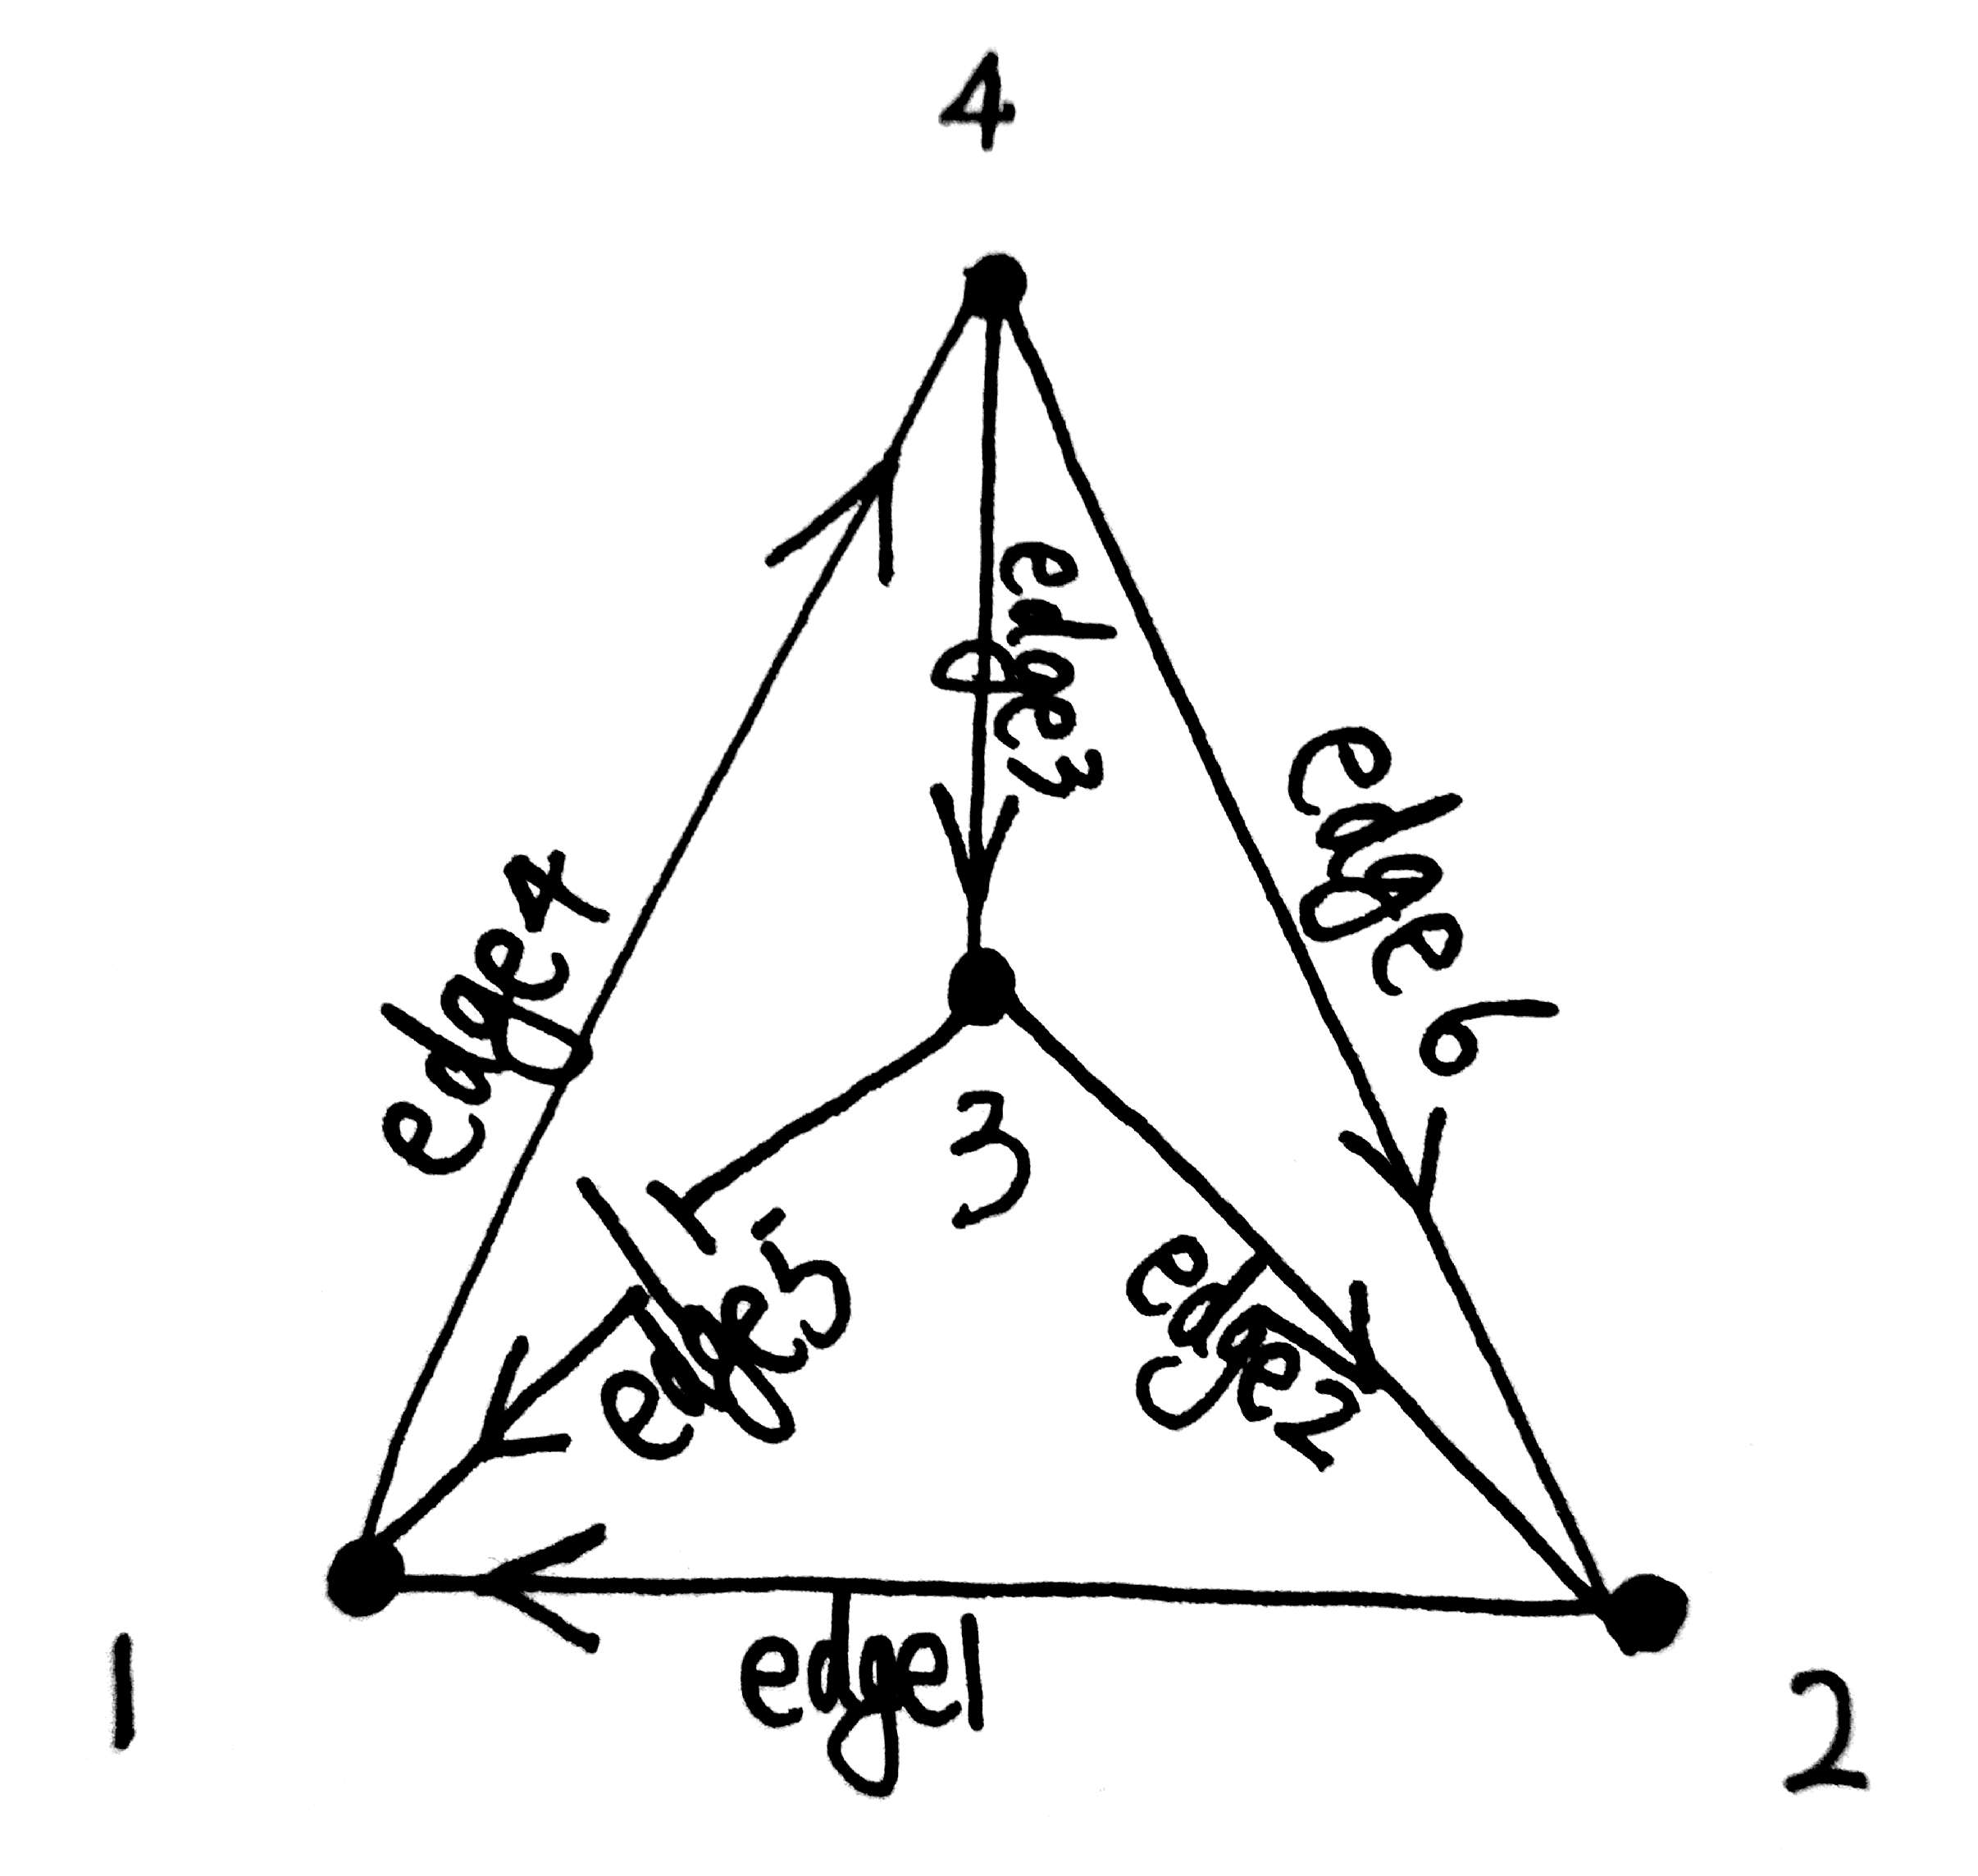
\includegraphics[width=0.8\textwidth]{1.png}
    \caption{ }
    \label{fig:2.5.16.1}
  \end{figure}
$$
\begin{pmatrix}
  1&0&0&-1&1&0\\
  -1&1&0&0&0&1\\
  0&-1&1&0&-1&0\\
  0&0&-1&1&0&-1
\end{pmatrix}
\begin{pmatrix}
  I_1\\
  I_2\\
  I_3\\
  I_4\\
  I_5\\
  I_6
\end{pmatrix}=
\begin{pmatrix}
  0\\
  0\\
  0\\
  0
\end{pmatrix}.
$$
设在节点1处的电位为$0$,则
$$
-\begin{pmatrix}
  1&-1&0&0\\
  0&1&-1&0\\
  0&0&1&-1\\
  -1&0&0&1\\
  1&0&-1&0\\
  0&1&0&-1
\end{pmatrix}
\begin{pmatrix}
  0\\
  P_2\\
  P_3\\
  P_4\\
\end{pmatrix}+
\begin{pmatrix}
  0\\
  0\\
  0\\
  0\\
  6\\
  0
\end{pmatrix}
=
\begin{pmatrix}
  I_1\times 1\\
  I_2\times 1\\
  I_3\times 1\\
  I_4\times 1\\
  I_5\times 1\\
  I_6\times 1
\end{pmatrix}
$$
联立解得
$$
\begin{pmatrix}
  I_1\\
  I_2\\
  I_3\\
  I_4\\
  I_5\\
  I_6
\end{pmatrix}=
\begin{pmatrix}
  -1.5\\
  -1.5\\
  1.5\\
  1.5\\
  3\\
  0\\
\end{pmatrix},
\begin{pmatrix}
  P_1\\
  P_2\\
  P_3\\
  P_4
\end{pmatrix}=
\begin{pmatrix}
  0\\
  -1.5\\
  -3\\
  -1.5\\
\end{pmatrix}.
$$
事实上,可以把上述两个线性方程组合并成一个线性方程组
$$
\begin{pmatrix}
  1&0&0&0&0&0&1&-1&0&0\\
  0&1&0&0&0&0&0&1&-1&0\\
  0&0&1&0&0&0&0&0&1&-1\\
  0&0&0&1&0&0&-1&0&0&1\\
  0&0&0&0&1&0&1&0&-1&0\\
  0&0&0&0&0&1&0&1&0&-1\\
  1&0&0&-1&1&0&0&0&0&0\\
  -1&1&0&0&0&1&0&0&0&0\\
  0&-1&1&0&-1&0&0&0&0&0\\
  0&0&-1&1&0&-1&0&0&0&0
\end{pmatrix}
\begin{pmatrix}
  I_1\\
  I_2\\
  I_3\\
  I_4\\
  I_5\\
  I_6\\
  P_{1}\\
  P_2\\
  P_3\\
  P_4\\
\end{pmatrix}=
\begin{pmatrix}
  0\\
  0\\
  0\\
  0\\
  6\\
  0\\
  0\\
  0\\
  0\\
  0
\end{pmatrix},
$$
解这个$10\times 10$线性方程组.过程如下:
\begin{align*}
  &  \begin{pmatrix}
    1&0&0&0&0&0&1&-1&0&0&0\\
    0&1&0&0&0&0&0&1&-1&0&0\\
    0&0&1&0&0&0&0&0&1&-1&0\\
    0&0&0&1&0&0&-1&0&0&1&0\\
    0&0&0&0&1&0&1&0&-1&0&6\\
    0&0&0&0&0&1&0&1&0&-1&0\\
    1&0&0&-1&1&0&0&0&0&0&0\\
    -1&1&0&0&0&1&0&0&0&0&0\\
    0&-1&1&0&-1&0&0&0&0&0&0\\
    0&0&-1&1&0&-1&0&0&0&0&0
  \end{pmatrix}\to\\&
                      \begin{pmatrix}
                        1&0&0&0&0&0&1&-1&0&0&0\\
                        0&1&0&0&0&0&0&1&-1&0&0\\
                        0&0&1&0&0&0&0&0&1&-1&0\\
                        0&0&0&1&0&0&-1&0&0&1&0\\
                        0&0&0&0&1&0&1&0&-1&0&6\\
                        0&0&0&0&0&1&0&1&0&-1&0\\
                        0&0&0&-1&1&0&-1&1&0&0&0\\
                        0&1&0&0&0&1&1&-1&0&0&0\\
                        0&-1&1&0&-1&0&0&0&0&0&0\\
                        0&0&-1&1&0&-1&0&0&0&0&0
                      \end{pmatrix}\to\\&
                                          \begin{pmatrix}
                                            1&0&0&0&0&0&1&-1&0&0&0\\
                                            0&1&0&0&0&0&0&1&-1&0&0\\
                                            0&0&1&0&0&0&0&0&1&-1&0\\
                                            0&0&0&1&0&0&-1&0&0&1&0\\
                                            0&0&0&0&1&0&1&0&-1&0&6\\
                                            0&0&0&0&0&1&0&1&0&-1&0\\
                                            0&0&0&-1&1&0&-1&1&0&0&0\\
                                            0&0&0&0&0&1&1&-2&1&0&0\\
                                            0&0&1&0&-1&0&0&1&-1&0&0\\
                                            0&0&-1&1&0&-1&0&0&0&0&0
                                          \end{pmatrix}\to\\&
                                                              \begin{pmatrix}
                                                                1&0&0&0&0&0&1&-1&0&0&0\\
                                                                0&1&0&0&0&0&0&1&-1&0&0\\
                                                                0&0&1&0&0&0&0&0&1&-1&0\\
                                                                0&0&0&1&0&0&-1&0&0&1&0\\
                                                                0&0&0&0&1&0&1&0&-1&0&6\\
                                                                0&0&0&0&0&1&0&1&0&-1&0\\
                                                                0&0&0&-1&1&0&-1&1&0&0&0\\
                                                                0&0&0&0&0&1&1&-2&1&0&0\\
                                                                0&0&0&0&-1&0&0&1&-2&1&0\\
                                                                0&0&0&1&0&-1&0&0&1&-1&0
                                                              \end{pmatrix}
                                                                                       \to\\&
                                                                                              \begin{pmatrix}
                                                                                                1&0&0&0&0&0&1&-1&0&0&0\\
                                                                                                0&1&0&0&0&0&0&1&-1&0&0\\
                                                                                                0&0&1&0&0&0&0&0&1&-1&0\\
                                                                                                0&0&0&1&0&0&-1&0&0&1&0\\
                                                                                                0&0&0&0&1&0&1&0&-1&0&6\\
                                                                                                0&0&0&0&0&1&0&1&0&-1&0\\
                                                                                                0&0&0&0&1&0&-2&1&0&1&0\\
                                                                                                0&0&0&0&0&1&1&-2&1&0&0\\
                                                                                                0&0&0&0&-1&0&0&1&-2&1&0\\
                                                                                                0&0&0&0&0&-1&1&0&1&-2&0
                                                                                              \end{pmatrix}
                                                                                                                       \to
\end{align*}
\begin{align*}
  &
    \begin{pmatrix}
      1&0&0&0&0&0&1&-1&0&0&0\\
      0&1&0&0&0&0&0&1&-1&0&0\\
      0&0&1&0&0&0&0&0&1&-1&0\\
      0&0&0&1&0&0&-1&0&0&1&0\\
      0&0&0&0&1&0&1&0&-1&0&6\\
      0&0&0&0&0&1&0&1&0&-1&0\\
      0&0&0&0&0&0&-3&1&1&1&-6\\
      0&0&0&0&0&1&1&-2&1&0&0\\
      0&0&0&0&0&0&1&1&-3&1&6\\
      0&0&0&0&0&-1&1&0&1&-2&0
    \end{pmatrix}\to\\&
                        \begin{pmatrix}
                          1&0&0&0&0&0&1&-1&0&0&0\\
                          0&1&0&0&0&0&0&1&-1&0&0\\
                          0&0&1&0&0&0&0&0&1&-1&0\\
                          0&0&0&1&0&0&-1&0&0&1&0\\
                          0&0&0&0&1&0&1&0&-1&0&6\\
                          0&0&0&0&0&1&0&1&0&-1&0\\
                          0&0&0&0&0&0&-3&1&1&1&-6\\
                          0&0&0&0&0&0&1&-3&1&1&0\\
                          0&0&0&0&0&0&1&1&-3&1&6\\
                          0&0&0&0&0&0&1&1&1&-3&0
                        \end{pmatrix}\to\\&
                                            \begin{pmatrix}
                                              1&0&0&0&0&0&1&-1&0&0&0\\
                                              0&1&0&0&0&0&0&1&-1&0&0\\
                                              0&0&1&0&0&0&0&0&1&-1&0\\
                                              0&0&0&1&0&0&-1&0&0&1&0\\
                                              0&0&0&0&1&0&1&0&-1&0&6\\
                                              0&0&0&0&0&1&0&1&0&-1&0\\
                                              0&0&0&0&0&0&-3&1&1&1&-6\\
                                              0&0&0&0&0&0&0&-\frac{8}{3}&\frac{4}{3}&\frac{4}{3}&-2\\
                                              0&0&0&0&0&0&0&\frac{4}{3}&-\frac{8}{3}&\frac{4}{3}&4\\
                                              0&0&0&0&0&0&0&\frac{4}{3}&\frac{4}{3}&-\frac{8}{3}&-2
                                            \end{pmatrix}\to\\&
                                                                \begin{pmatrix}
                                                                  1&0&0&0&0&0&1&-1&0&0&0\\
                                                                  0&1&0&0&0&0&0&1&-1&0&0\\
                                                                  0&0&1&0&0&0&0&0&1&-1&0\\
                                                                  0&0&0&1&0&0&-1&0&0&1&0\\
                                                                  0&0&0&0&1&0&1&0&-1&0&6\\
                                                                  0&0&0&0&0&1&0&1&0&-1&0\\
                                                                  0&0&0&0&0&0&-3&1&1&1&-6\\
                                                                  0&0&0&0&0&0&0&-\frac{8}{3}&\frac{4}{3}&\frac{4}{3}&-2\\
                                                                  0&0&0&0&0&0&0&0&-2&2&3\\
                                                                  0&0&0&0&0&0&0&0&2&-2&-3
                                                                \end{pmatrix}\to\\&
                                                                                    \begin{pmatrix}
                                                                                      1&0&0&0&0&0&1&-1&0&0&0\\
                                                                                      0&1&0&0&0&0&0&1&-1&0&0\\
                                                                                      0&0&1&0&0&0&0&0&1&-1&0\\
                                                                                      0&0&0&1&0&0&-1&0&0&1&0\\
                                                                                      0&0&0&0&1&0&1&0&-1&0&6\\
                                                                                      0&0&0&0&0&1&0&1&0&-1&0\\
                                                                                      0&0&0&0&0&0&-3&1&1&1&-6\\
                                                                                      0&0&0&0&0&0&0&-\frac{8}{3}&\frac{4}{3}&\frac{4}{3}&-2\\
                                                                                      0&0&0&0&0&0&0&0&-2&2&3\\
                                                                                      0&0&0&0&0&0&0&0&0&0&0
                                                                                    \end{pmatrix}
\end{align*}
令$P_4$为自由变量,不妨设$P_4=-1.5$,则由$-2P_3+2P_4=3$,可得$P_3=-3$.再
由$-\frac{8}{3}P_2+\frac{4}{3}P_3+\frac{4}{3}P_4=-2$,可得$P_2=-1.5$.就
这样子逐步做下去,可以解得$I_1,I_2,\cdots,I_6$和$P_1,P_2,P_3,P_4$.
\end{solution}
\section{子空间对与矩阵的乘积}
\begin{question}
  在全体$4\times 4$矩阵所成空间中,取三对角矩阵子空间为$V$,取上三角矩阵
  子空间为$W$.试描述子空间$V+W$和$V\cap W$.$V+W$的成员是上Hessenberg矩
  阵,请验证公式(21).
\end{question}
\begin{solution}
  $V+W$的维数是$13$.$V\cap W$的维数是$7$.$V$的维数是$10$,$W$的维数
  是$10$.可见,确实有
$$
\dim (V+W)+\dim (V\cap W)=\dim V+\dim W.
$$
\end{solution}
\begin{question}
  略.因为这道题目几乎完全是在陈述,不太需要解答.
\end{question}
\begin{question}
  $V$由$v_1=(1,1,0,0)$,$v_2=(1,0,1,0)$张
  成,$W$由$w_1=(0,1,0,1)$,$w_2=(0,0,1,1)$张成.试求和$V+W$的基底,并求
  出$V\cap W$的维数和基底.
\end{question}
\begin{solution}
  考察矩阵
$$
A=
\begin{pmatrix}
  1&1&0&0\\
  1&0&1&0\\
  0&1&0&1\\
  0&0&1&1
\end{pmatrix}.
$$
为了求$V+W$的基底,对矩阵$A$进行基本行变换.
$$
  \begin{pmatrix}
    1&1&0&0\\
    1&0&1&0\\
    0&1&0&1\\
    0&0&1&1
  \end{pmatrix}\to
  \begin{pmatrix}
    1&1&0&0\\
    0&-1&1&0\\
    0&1&0&1\\
    0&0&1&1
  \end{pmatrix}\to
  \begin{pmatrix}
    1&1&0&0\\
    0&-1&1&0\\
    0&0&1&1\\
    0&0&1&1
  \end{pmatrix}\to
  \begin{pmatrix}
    1&1&0&0\\
    0&-1&1&0\\
    0&0&1&1\\
    0&0&0&0
  \end{pmatrix}.
$$
所以$V+W$的一组基底为
$$
\begin{pmatrix}
  1\\
  1\\
  0\\
  0\\
\end{pmatrix},
\begin{pmatrix}
  1\\
  0\\
  1\\
  0
\end{pmatrix},
\begin{pmatrix}
  0\\
  1\\
  0\\
  1
\end{pmatrix}.
$$
下面求$V\cap W$的基底.设
$$
\begin{pmatrix}
  x_1\\
  x_2\\
  x_3\\
  x_4
\end{pmatrix}\in V\cap W,
$$
则存在$\alpha,\beta,m,n$,使得
$$
\begin{pmatrix}
  x_1\\
  x_2\\
  x_3\\
  x_4
\end{pmatrix}=\alpha
\begin{pmatrix}
  1\\
  1\\
  0\\
  0
\end{pmatrix}+\beta
\begin{pmatrix}
  1\\
  0\\
  1\\
  0
\end{pmatrix}=m
\begin{pmatrix}
  0\\
  1\\
  0\\
  1
\end{pmatrix}+n
\begin{pmatrix}
  0\\
  0\\
  1\\
  1
\end{pmatrix},
$$
即
$$
\begin{pmatrix}
  1&1&0&0\\
  1&0&1&0\\
  0&1&0&1\\
  0&0&1&1
\end{pmatrix}
\begin{pmatrix}
  \alpha\\
  \beta\\
  -m\\
  -n
\end{pmatrix}=
\begin{pmatrix}
  0\\
  0\\
  0\\
  0
\end{pmatrix},
$$
即
$$
\begin{pmatrix}
  1&1&0&0\\
  0&-1&1&0\\
  0&0&1&1\\
  0&0&0&0
\end{pmatrix}
\begin{pmatrix}
  \alpha\\
  \beta\\
  -m\\
  -n
\end{pmatrix}=
\begin{pmatrix}
  0\\
  0\\
  0\\
  0
\end{pmatrix}.
$$
可得$n$是自由变量.令$n=1$,可得
$$
m=-1,\beta=1,\alpha=-1.
$$
因此$V\cap W$的维数为$1$,一组基底为$
\begin{pmatrix}
  0\\
  -1\\
  1\\
  0
\end{pmatrix}.  $
\end{solution}
\begin{question}
  假定$V$是由分量为$(1,1,0,1)$和$(1,2,0,0)$的列向量张成的.试求子空
  间$W$,使得$V\oplus W=\mathbf{R}^4$.记号的意义见练习2.6.2.
\end{question}
\begin{solution}
  我们尝试求出$V$在$\mathbf{R}^4$中的正交
  补$V^{\perp}$.设$(x_1,x_2,x_3,x_4)\in V^{\perp}$.则
$$
\begin{pmatrix}
  1&1&0&1\\
  1&2&0&0
\end{pmatrix}
\begin{pmatrix}
  x_1\\
  x_2\\
  x_3\\
  x_4
\end{pmatrix}=
\begin{pmatrix}
  0\\
  0\\
\end{pmatrix}.
$$
化成
$$
\begin{pmatrix}
  1&1&0&1\\
  0&1&0&-1
\end{pmatrix}
\begin{pmatrix}
  x_1\\
  x_2\\
  x_3\\
  x_4
\end{pmatrix}=
\begin{pmatrix}
  0\\
  0
\end{pmatrix}.
$$
可见,$x_3,x_4$是自由变量,$x_1,x_2$是主变量.当$x_3=1,x_4=0$时,解
得$x_1=0,x_2=0$.当$x_3=0,x_4=1$时,$x_1=-2,x_2=1$.因此可得$W$的一组基是
$$
\begin{pmatrix}
  0\\
  0\\
  1\\
  0
\end{pmatrix},
\begin{pmatrix}
  -2\\
  1\\
  0\\
  1
\end{pmatrix},
$$
$W$就由这两个向量张成.
\end{solution}
\begin{question}
  验证“$V\cap
  W$中的每一个$y$都来自$\mathcal{N}(Q)$中唯一的一个$x$”.试对给定
  的$y$给出求唯一可能的$x$的方法.
\end{question}
\begin{solution}
  对于$V\cap
  W$中的每一个$y$,它既是$V$中的向量,又是$W$中的向量.因此它既能被$V$的
  基底进行唯一的线性表示,又能被$W$中的基底进行唯一的线性表示.设
$$
y=a_1v_1+a_2v_2+\cdots+a_nv_n=b_1w_1+b_2w_2+\cdots+b_mw_m,
$$
其中$v_1,\cdots,v_n$是$n$维线性空间$V$的基底,$w_1,\cdots,w_m$是$m$维线
性空间$W$的基底.因此$y$来自$\mathcal{N}(Q)$中的唯一一个向
量$(a_1,a_2,\cdots,a_n,-b_1,-b_2,\cdots,-b_m)$.
\end{solution}
\begin{question}
  试举例证明:(i)$AB$的化零空间不一定包含$A$的化零空间,(ii)$AB$的列空间
  不一定含于$B$的列空间.
\end{question}
\begin{solution}
  \begin{itemize}
  \item 令矩阵$A=
    \begin{pmatrix}
      1&0\\
      0&0
    \end{pmatrix}, $矩阵$B=
    \begin{pmatrix}
      0&1\\
      1&0
    \end{pmatrix}.  $则矩阵$AB=
    \begin{pmatrix}
      0&1\\
      0&0
    \end{pmatrix},
    $矩阵$AB$的化零空间是$(1,0)$张成的,矩阵$A$的化零空间是$(0,1)$张成
    的,可见$AB$的化零空间不一定包含$A$的化零空间.
  \item 令矩阵$B=
    \begin{pmatrix}
      1&0\\
      0&0
    \end{pmatrix}, $矩阵$A=
    \begin{pmatrix}
      0&1\\
      1&0
    \end{pmatrix}, $则$AB=
    \begin{pmatrix}
      0&1\\
      0&0
    \end{pmatrix}.  $可见,矩阵$AB$的列空间不一定含于矩阵$B$的列空间.
  \end{itemize}
\end{solution}
\begin{question}
  试证对于有很多元素为零的矩阵,$v(AB)$可以小于$v(A)$.
\end{question}
\begin{solution}
  令矩阵$A=
  \begin{pmatrix}
    1&1&1&1&1\\
    0&0&0&0&0
  \end{pmatrix}, $矩阵$B=
  \begin{pmatrix}
    0\\
    0\\
    0\\
    0\\
    0
  \end{pmatrix}.  $可得矩阵$AB=
  \begin{pmatrix}
    0\\
    0
  \end{pmatrix}.  $于是$v(AB)=1$,$v(A)=5$.
\end{solution}
\begin{question}
  试将矩阵
$$
A=
\begin{pmatrix}
  0&1&4&0\\
  0&2&8&0
\end{pmatrix}
$$
分解为$A=\overline{L}\overline{U}$,并验证$\overline{L}$的列是$A$的列空
间的基底.
\end{question}
\begin{solution}
  首先,
$$
\begin{pmatrix}
  1&0\\
  -2&1
\end{pmatrix}
\begin{pmatrix}
  0&1&4&0\\
  0&2&8&0
\end{pmatrix}=
\begin{pmatrix}
  0&1&4&0\\
  0&0&0&0
\end{pmatrix}.
$$
可见,
$$
A=
\begin{pmatrix}
  0&1&4&0\\
  0&2&8&0
\end{pmatrix}=
\begin{pmatrix}
  1&0\\
  2&1
\end{pmatrix}
\begin{pmatrix}
  0&1&4&0\\
  0&0&0&0
\end{pmatrix}=
\begin{pmatrix}
  1\\
  2
\end{pmatrix}
\begin{pmatrix}
  0&1&4&0
\end{pmatrix}.
$$
$
\begin{pmatrix}
  1\\
  2
\end{pmatrix}
$确实是$A$的列空间的基底.
\end{solution}
\begin{question}
  将矩阵换成
$$
A=
\begin{pmatrix}
  0&0\\
  1&2\\
  4&8\\
  0&0
\end{pmatrix}
$$
再做上一题,这里用到置换矩阵$P$.
\end{question}
\begin{solution}
  $$ 
  \begin{pmatrix}
    1&0&0&0\\
    0&1&0&0\\
    -4&0&1&0\\
    0&0&0&1
  \end{pmatrix}
  \begin{pmatrix}
    0&1&0&0\\
    1&0&0&0\\
    0&0&1&0\\
    0&0&0&1
  \end{pmatrix}
  \begin{pmatrix}
    0&0\\
    1&2\\
    4&8\\
    0&0
  \end{pmatrix}=
  \begin{pmatrix}
    1&2\\
    0&0\\
    0&0\\
    0&0
  \end{pmatrix}.
 $$
 可见,
 \begin{align*}
   A&=
      \begin{pmatrix}
        0&1&0&0\\
        1&0&0&0\\
        0&0&1&0\\
        0&0&0&1
      \end{pmatrix}
               \begin{pmatrix}
                 1&0&0&0\\
                 0&1&0&0\\
                 4&0&1&0\\
                 0&0&0&1
               \end{pmatrix}
                        \begin{pmatrix}
                          1&2\\
                          0&0\\
                          0&0\\
                          0&0
                        \end{pmatrix}=
                             \begin{pmatrix}
                               0&1&0&0\\
                               1&0&0&0\\
                               4&0&1&0\\
                               0&0&0&1
                             \end{pmatrix}
                                      \begin{pmatrix}
                                        1&2\\
                                        0&0\\
                                        0&0\\
                                        0&0\\
                                      \end{pmatrix}
   \\&=
       \begin{pmatrix}
         0\\
         1\\
         4\\
         0
       \end{pmatrix}
   \begin{pmatrix}
     1&2
   \end{pmatrix}.
 \end{align*}
\end{solution}
\begin{question}
  $\overline{L}$的每一列乘以$\overline{U}$的对应的行,这样即可
  将$A=\overline{L}\overline{U}$化为秩为$1$的$r$个矩阵的和.矩阵
$$
A=
\begin{pmatrix}
  1&3&3&2\\
  2&6&9&5\\
  -1&-3&3&0
\end{pmatrix}
$$
的秩为$2$.试构造出它的$\overline{L}$和$\overline{U}$,将它分解为$r$个秩
为$1$的矩阵的和.
\end{question}
\begin{solution}
$$
\begin{pmatrix}
  1&0&0\\
  0&1&0\\
  0&-2&1
\end{pmatrix}
\begin{pmatrix}
  1&0&0\\
  0&1&0\\
  1&0&1
\end{pmatrix}
\begin{pmatrix}
  1&0&0\\
  -2&1&0\\
  0&0&1
\end{pmatrix}
\begin{pmatrix}
  1&3&3&2\\
  2&6&9&5\\
  -1&-3&3&0
\end{pmatrix}=
\begin{pmatrix}
  1&3&3&2\\
  0&0&3&1\\
  0&0&0&0
\end{pmatrix},
$$
所以
\begin{align*}
  A&=
     \begin{pmatrix}
       1&3&3&2\\
       2&6&9&5\\
       -1&-3&3&0
     \end{pmatrix}=
                \begin{pmatrix}
                  1&0&0\\
                  2&1&0\\
                  0&0&1
                \end{pmatrix}
                       \begin{pmatrix}
                         1&0&0\\
                         0&1&0\\
                         -1&0&1
                       \end{pmatrix}
                               \begin{pmatrix}
                                 1&0&0\\
                                 0&1&0\\
                                 0&2&1
                               \end{pmatrix}
                                      \begin{pmatrix}
                                        1&3&3&2\\
                                        0&0&3&1\\
                                        0&0&0&0
                                      \end{pmatrix}\\&=
                                                       \begin{pmatrix}
                                                         1&0&0\\
                                                         2&1&0\\
                                                         -1&2&1
                                                       \end{pmatrix}
                                                               \begin{pmatrix}
                                                                 1&3&3&2\\
                                                                 0&0&3&1\\
                                                                 0&0&0&0
                                                               \end{pmatrix}=
                                                                        \begin{pmatrix}
                                                                          1&0\\
                                                                          2&1\\
                                                                          -1&2
                                                                        \end{pmatrix}
                                                                              \begin{pmatrix}
                                                                                1&3&3&2\\
                                                                                0&0&3&1
                                                                              \end{pmatrix}
  \\&=
      \begin{pmatrix}
        1\\
        2\\
        -1
      \end{pmatrix}
  \begin{pmatrix}
    1&3&3&2
  \end{pmatrix}+
           \begin{pmatrix}
             0\\
             1\\
             2
           \end{pmatrix}
  \begin{pmatrix}
    0&0&3&1
  \end{pmatrix}
  \\&=
      \begin{pmatrix}
        1&3&3&2\\
        2&6&6&4\\
        -1&-3&-3&-2
      \end{pmatrix}+
                  \begin{pmatrix}
                    0&0&0&0\\
                    0&0&3&1\\
                    0&0&6&2
                  \end{pmatrix}.
\end{align*}
\end{solution}
\begin{question}
  求$A=
  \begin{pmatrix}
    1&2&3\\
    3&6&9
  \end{pmatrix}
  $的最大可逆子矩阵和秩.
\end{question}
\begin{solution}
  最大可逆子矩阵是
$$
\begin{pmatrix}
  1
\end{pmatrix},
$$
秩为$1$.
\end{solution}
\begin{question}
  设$A,B$分别为$m\times n$和$n\times m$矩阵,$n<m$.试证它们的积$AB$是奇
  异的.
\end{question}
\begin{solution}
  $AB$是$m\times m$矩阵.但是$r(AB)\leq r(A)\leq n<m$,因此$AB$是奇异矩阵.
\end{solution}
\begin{question}
  试证$(A+B)$的秩$\leq A$的秩+$B$的秩.
\end{question}
\begin{solution}
  设矩阵$A$的列空间为$W$,矩阵$B$的列空间为$V$.则矩阵$A+B$的列空间含
  于$W\cup V$.因此矩阵$A+B$的列空间的维数(即秩)不大于$\dim (W\cup
  V)$.而$\dim (W\cup V)\leq \dim W+\dim V
  $,因此$(A+B)$的秩$\leq A$的秩+$B$的秩.
\end{solution}
\begin{question}
  设$\mathcal{N}(AB)=\mathcal{N}(B)$,又设向量$y$既属
  于$\mathcal{R}(B)$又属于$\mathcal{N}(A)$.试证$y=0$.
\end{question}
\begin{solution}
  如果存在非零向量$y\in \mathcal{R}(B)\cap \mathcal{N}(A)$,则必定存在向
  量$x$,使得$y=B(x)$.且$\mathcal{N}(B)+\{x\}\subset \mathcal{N}(AB)$.并
  且$\dim (\mathcal{N}(B)+\{x\})=\dim (\mathcal{N}(B)+1$,这表
  明$\dim(\mathcal{N}(AB))\geq
  \dim(\mathcal{N}(B)+1$,这与$\mathcal{N}(AB)=\mathcal{N}(B)$矛盾.可见,
  假设不成立,即原命题成立.
\end{solution}
\begin{question}
  设$A$为可逆方阵,试证$AB$的化零空间、行空间和秩都同于$B$.
\end{question}
\begin{solution}
  \begin{itemize}
  \item 首先$AB$的化零空间同于$B$的化零空间.这是因为,首
    先,$\mathcal{N}(B)\subset \mathcal{N}(AB)$.因此我们只用再证
    明$\mathcal{N}(AB)\subset
    \mathcal{N}(B)$即可.如果向量$x$位于$AB$的化零空间,即满
    足$AB(x)=0$,则$A(B(x))=0$,由于$A$是可逆矩阵,因此$B(x)=0$,可见$x$也
    位于$B$的化零空间.因此$\mathcal{N}(AB)\subset \mathcal{N}(B)$.综上
    所述,$\mathcal{N}(AB)=\mathcal{N}(B)$.
  \item
    首先,易得$AB$的行空间含于$B$的行空间.只用证明$B$的行空间也含
    于$AB$的行空间即可.对于$B$的行空间的任意一个向量$y$,必定存在向
    量$x$,使得$xB=y$.由于矩阵$A$可逆,因此必定存在向量$m$,使得$mA=x$.可
    见,$m(AB)=y$,所以$y$在矩阵$AB$的行空间里.于是$B$的行空间也含于矩
    阵$AB$的行空间.综上所述,矩阵$AB$的行空间等于矩阵$B$的行空间.
  \item 既然行空间相等,因此行秩相等,即矩阵的秩相等.
  \end{itemize}
\end{solution}
\begin{question}
  考虑由全体$2\times 2$矩阵$B$所组成的四维向量空间$V$.设$A$是一个特殊的
  矩阵,按每一个$2\times
  2$矩阵$B$都被变成$AB$这样的方式进行变换,则$V$变成它自己.如果$A$可逆,
  则该变换没有化零空间,唯一被变成零的矩阵$(AB=0)$是矩阵$B=0$.
  \begin{itemize}
  \item 设$A=
    \begin{pmatrix}
      1&0\\
      2&0
    \end{pmatrix}
    $,试求该变换的化零空间(满足$AB=0$的所有的$B$所成的空间),并求出它的
    维数(即变换的零度,而不是$A$的零度).
  \item 求出该变换的值域,并计算出该值域的维数,再验证秩+零度=$V$的维数.
  \end{itemize}
\end{question}
\begin{solution}
  \begin{itemize}
  \item 设矩阵$B=
    \begin{pmatrix}
      a&b\\
c&d
    \end{pmatrix}
$,$AB=0$即
$$
\begin{pmatrix}
  1&0\\
2&0
\end{pmatrix}
\begin{pmatrix}
  a&b\\
c&d
\end{pmatrix}=
\begin{pmatrix}
  0&0\\
0&0
\end{pmatrix},
$$
即
$$
a=b=0.
$$
可见该变换的化零空间为$\left\{
  \begin{pmatrix}
    0&0\\
c&d
  \end{pmatrix}:c,d\in \mathbf{R}
\right\}$,变换的零度为$2$.
\item 变换的值域是
$$
\left\{
  \begin{pmatrix}
    a&b\\
2a&2b
  \end{pmatrix}:a,b\in \mathbf{R}
\right\}.
$$
值域的维数是$2$.我们发现,变换的零度加上变换的值域等于$4$,恰好是$V$的
维数.
  \end{itemize}
\end{solution}
\section{复习题}
\begin{question}
  求$\mathbf{R}^4$的子空间的基底,子空间中$x_1=x_2=x_3$.
\end{question}
\begin{solution}
  该子空间的一组基底为$(1,1,1,0),(0,0,0,1)$.
\end{solution}
\begin{question}
  $$ 
  A=
  \begin{pmatrix}
    1&2&0&2&1\\
    -1&-2&1&1&0\\
    1&2&-8&-7&-2
  \end{pmatrix}
 $$
 试求出$A$的阶梯阵$U$和四个基本子空间的维数.
\end{question}
\begin{solution}
  将矩阵$A$进行初等行变换.
$$
\begin{pmatrix}
  1&2&0&2&1\\
  -1&-2&1&1&0\\
  1&2&-8&-7&-2
\end{pmatrix}\to
\begin{pmatrix}
  1&2&0&2&1\\
  0&0&1&3&1\\
  0&0&-8&-9&-3
\end{pmatrix}\to
\begin{pmatrix}
  1&2&0&2&1\\
  0&0&1&3&1\\
  0&0&0&15&5
\end{pmatrix}.
$$这样就得到了$A$的阶梯型矩阵$U$.从中可得$\dim \mathcal{N}(A)=2$.矩阵
$A$的行空间和列空间维数都是$3$.且$A$的左化零空间的维数是$1$.
\end{solution}
\begin{question}
  用给出基底的方法写出$\mathbf{R}^3$的二维子空间,要求其中不包含向
  量$(1,0,0),(0,1,0),(0,0,1)$中的任何一个.
\end{question}
\begin{solution}
  $\mathbf{R}^3$的一个二维子空间为$\{(1,1,0)\}+\{(0,1,1)\}$.
\end{solution}
\begin{question}
  试求出$A$的秩和化零空间
$$
A=
\begin{pmatrix}
  0&0&1\\
  0&0&1\\
  1&1&1
\end{pmatrix}.
$$
\end{question}
\begin{solution}
  $A$秩显然为$2$.下面求出$A$的化零空间.
$$
\begin{pmatrix}
  0&0&1\\
  0&0&1\\
  1&1&1
\end{pmatrix}\to
\begin{pmatrix}
  1&1&1\\
  0&0&1\\
  0&0&1
\end{pmatrix}\to
\begin{pmatrix}
  1&1&1\\
  0&0&1\\
  0&0&0
\end{pmatrix}
$$
所以矩阵$A$的化零空间的一组基底为
$$
\begin{pmatrix}
  -1\\
  1\\
  0\\
\end{pmatrix}.
$$
\end{solution}
\begin{question}
  构造一个矩阵,其化零空间由$
  \begin{pmatrix}
    1&0&1
  \end{pmatrix}^T $张成.
\end{question}
\begin{solution}
$$
  \begin{pmatrix}
    0&0&0\\
    0&1&0\\
    0&0&0
  \end{pmatrix}.
$$
\end{solution}
\begin{question}
  判断下列各条成立否,不成立的请举出反例.
  \begin{itemize}
  \item 如果向量$x_1,\cdots,x_m$生成子空间$S$,则$S$的维数为$m$.
  \item 向量空间的两个子空间的交不能是空的.
  \item 若$Ax=Ay$,则$x=y$.
  \item $A$的行空间有唯一的基底,可以用化$A$为阶梯阵的方式求出来.
  \item 若方阵$A$的列线性无关,则$A^2$的列也线性无关.
  \end{itemize}
\end{question}
\begin{solution}
  \begin{itemize}
  \item 错.如果向量$x_1,\cdots,x_m$是线性相关的,则$S$的维数小于$m$.
  \item 对.至少有一个公共元素零向量.
  \item 错.令$A$为零矩阵,且$x\neq y$,即为反例.
  \item 错.
  \item 对.只用证明$A^2x=0$只有唯一解即可,也即证明$Ax=A^{-1}0=0$只有唯
    一解.由于$A$是可逆的,因此成立.
  \end{itemize}
\end{solution}
\begin{question}
  试求出$A,B,C$它们各自的四个基本子空间的基底.
$$
A=
\begin{pmatrix}
  1&2\\
  3&6
\end{pmatrix},B=
\begin{pmatrix}
  0&0\\
  0&0
\end{pmatrix},C=
\begin{pmatrix}
  1&1&0&0\\
  0&1&0&1
\end{pmatrix}.
$$
\end{question}
\begin{solution}
  \begin{itemize}
  \item $A$的行空间的一个基底为$(1,2)$,列空间的一个基底为$
    \begin{pmatrix}
      1\\
      3
    \end{pmatrix}
    $.$A$的化零空间的一个基底是$
    \begin{pmatrix}
      -2\\
      1
    \end{pmatrix}.  $而且,$A$的左化零空间的一个基底是$
    \begin{pmatrix}
      -3&1
    \end{pmatrix}.  $
  \item $B$的列空间的一组基底是$\emptyset$.化零空间的一组基底是$
    \begin{pmatrix}
      1\\
      0
    \end{pmatrix},
    \begin{pmatrix}
      0\\
      1
    \end{pmatrix}.  $行空间的一组基底是$\emptyset$,左化零空间的一组基底
    是$
    \begin{pmatrix}
      0&1
    \end{pmatrix},
    \begin{pmatrix}
      1&0
    \end{pmatrix}.  $
  \item 矩阵$C$的列空间的一组基底是
$$
\begin{pmatrix}
  1\\
  0\\
\end{pmatrix},
\begin{pmatrix}
  0\\
  1
\end{pmatrix}.
$$化零空间的一组基底是
$$
\begin{pmatrix}
  0\\
  0\\
  1\\
  0\\
\end{pmatrix},
\begin{pmatrix}
  1\\
  -1\\
  0\\
  1\\
\end{pmatrix}.
$$矩阵$C$行空间的一组基底是$
\begin{pmatrix}
  1&1&0&0
\end{pmatrix},
\begin{pmatrix}
  0&1&0&1
\end{pmatrix}.  $左化零空间的一组基底是$\emptyset$.
\end{itemize}
\end{solution}
\begin{question}
  求出$u+v+w=1,u-w=2$的通解.
\end{question}
\begin{solution}
  易求得通解为
$$
\begin{pmatrix}
  2\\
  -1\\
  0
\end{pmatrix}+w
\begin{pmatrix}
  1\\
  -2\\
  1
\end{pmatrix}
$$
\end{solution}
\begin{question}
  其行空间包含$
  \begin{pmatrix}
    1&1&1
  \end{pmatrix}^T $,其化零空间包含$
  \begin{pmatrix}
    1&0&0
  \end{pmatrix}^T $.问这样的矩阵存在否?
\end{question}
\begin{solution}
  不存在.因为行空间中的所有向量与化零空间中的所有向量都要正交.
\end{solution}
\begin{question}
  求出正交于$
  \begin{pmatrix}
    1&4&4&1
  \end{pmatrix}
  $和$
  \begin{pmatrix}
    2&9&8&2
  \end{pmatrix}
  $的所有向量.
\end{question}
\begin{solution}
  正交于如上向量的向量设为$
  \begin{pmatrix}
    x\\
    y\\
    z\\
    w
  \end{pmatrix}
  $.则有
$$
\begin{pmatrix}
  1&4&4&1\\
  2&9&8&2
\end{pmatrix}
\begin{pmatrix}
  x\\
  y\\
  z\\
  w
\end{pmatrix}=
\begin{pmatrix}
  0\\
  0
\end{pmatrix}.
$$
化为
$$
\begin{pmatrix}
  1&4&4&1\\
  0&1&0&0
\end{pmatrix}
\begin{pmatrix}
  x\\
  y\\
  z\\
  w
\end{pmatrix}=
\begin{pmatrix}
  0\\
  0
\end{pmatrix}.
$$
把$x,y$作为主变量,把$z,w$当自由变量.可得正交于题干中的两个向量的所有向
量形成的子空间的一组基底是
$$
\begin{pmatrix}
  -4\\
  0\\
  1\\
  0\\
\end{pmatrix},
\begin{pmatrix}
  -1\\
  0\\
  0\\
  1\\
\end{pmatrix}.
$$
\end{solution}
\begin{question}
  向量$(1,2,1),(0,1,3),(3,7,6)$是否位于$\mathbf{R}^3$中的同一张平面上?
  如果是,请求出正交于这张平面的一个向量.
\end{question}
\begin{solution}
  我们先判断这三个向量是否是线性相关的.为此调查矩阵
$$
A=
\begin{pmatrix}
  1&2&1\\
  0&1&3\\
  3&7&6
\end{pmatrix}
$$
将矩阵$A$进行初等行变换,可得
$$
\begin{pmatrix}
  1&2&1\\
  0&1&3\\
  3&7&6
\end{pmatrix}\to
\begin{pmatrix}
  1&2&1\\
  0&1&3\\
  0&1&3
\end{pmatrix}\to
\begin{pmatrix}
  1&2&1\\
  0&1&3\\
  0&0&0
\end{pmatrix}.
$$
可见,这三个向量线性相关,即位于同一张平面上.下面求出正交于这张平面的一
个向量,设这个向量是$
\begin{pmatrix}
  x\\
  y\\
  z
\end{pmatrix}, $则
$$
\begin{pmatrix}
  1&2&1\\
  0&1&3\\
  0&0&0
\end{pmatrix}
\begin{pmatrix}
  x\\
  y\\
  z
\end{pmatrix}=
\begin{pmatrix}
  0\\
  0\\
  0
\end{pmatrix}.
$$
可得$
\begin{pmatrix}
  x\\
  y\\
  z
\end{pmatrix}
$可以等于$
\begin{pmatrix}
  5\\
  -3\\
  1\\
\end{pmatrix}.  $
\end{solution}
\begin{question}
  $Ax=b$.问当且仅当$b$正交于四个基本子空间中哪一个时,该方程组才有解.
\end{question}
\begin{solution}
  当$b$正交于矩阵$A$的左化零空间时,$b$必定位于左化零空间的正交补,
  即$b$位于矩阵$A$的列空间,此时方程组有解;反之,当方程组有解时,$b$位于
  矩阵$A$的列空间,即位于左化零空间的正交补,所以$b$正交于左化零空间.
\end{solution}
\begin{question}
  试求出下列方程组的所有解
$$
\begin{pmatrix}
  1&1&1\\
  2&1&1\\
  3&1&1
\end{pmatrix}
\begin{pmatrix}
  x_1\\
  x_2\\
  x_3
\end{pmatrix}=
\begin{pmatrix}
  2\\
  3\\
  4
\end{pmatrix},
\begin{pmatrix}
  1&1&1\\
  2&1&1\\
  3&1&1
\end{pmatrix}
\begin{pmatrix}
  x_1\\
  x_2\\
  x_3
\end{pmatrix}=
\begin{pmatrix}
  2\\
  3\\
  5
\end{pmatrix}.
$$
\end{question}
\begin{solution}
  \begin{itemize}
  \item
$$
\begin{pmatrix}
  1&1&1&2\\
  2&1&1&3\\
  3&1&1&4
\end{pmatrix}\to
\begin{pmatrix}
  1&1&1&2\\
  0&-1&-1&-1\\
  0&-2&-2&-2
\end{pmatrix}\to
\begin{pmatrix}
  1&1&1&2\\
  0&-1&-1&-1\\
  0&0&0&0
\end{pmatrix}.
$$
解方程组
$$
\begin{pmatrix}
  1&1&1\\
  0&-1&-1\\
  0&0&0
\end{pmatrix}
\begin{pmatrix}
  x_1\\
  x_2\\
  x_3
\end{pmatrix}=
\begin{pmatrix}
  2\\
  -1\\
  0
\end{pmatrix}
$$
可得通解为
$$
\begin{pmatrix}
  1\\
  1\\
  0
\end{pmatrix}+x_3
\begin{pmatrix}
  0\\
  -1\\
  1
\end{pmatrix}.
$$
\item
$$
\begin{pmatrix}
  1&1&1&2\\
  2&1&1&3\\
  3&1&1&5
\end{pmatrix}\to
\begin{pmatrix}
  1&1&1&2\\
  0&-1&-1&-1\\
  0&-2&-2&-1
\end{pmatrix}\to
\begin{pmatrix}
  1&1&1&2\\
  0&-1&-1&-1\\
  0&0&0&1
\end{pmatrix}.
$$
解方程组
$$
\begin{pmatrix}
  1&1&1\\
  0&-1&-1\\
  0&0&0
\end{pmatrix}
\begin{pmatrix}
  x_1\\
  x_2\\
  x_3
\end{pmatrix}=
\begin{pmatrix}
  2\\
  -1\\
  1
\end{pmatrix}
$$
可得无解.
\end{itemize}
\end{solution}
\begin{question}
  向量$(1,1,3),(2,3,6),$
\end{question}
\begin{solution}
  
\end{solution}
\begin{question}
  试求出矩阵$A$,使$Ax=b$的解的个数为
  \begin{itemize}
  \item $0$或$1$,决定于$b$
  \item $1$或$\infty$,决定于$b$
  \item $0$或$\infty$,决定于$b$
  \item $1$,与$b$无关.
  \end{itemize}
\end{question}
\begin{solution}
  如果矩阵$A$的秩小于行数,且小于列数,则$Ax=b$是否有解取决于向量$b$.若$b$属于$A$的列空间,则有解,且有无穷多个解;若$b$不属于$A$的列空间,则无解.\\

  如果$A$的秩小于行数,且等于列数,则$Ax=b$是否有解取决于向量$b$.当$b$属于$A$的列空间时,有唯一解;$b$不属于$A$的列空间时,无解.\\

  如果$A$的秩等于行数,且小于列数,则$Ax=b$必有无穷多个解.\\

  如果$A$的秩等于行数且等于列数,则$Ax=b$必有唯一解.
  \begin{itemize}
  \item 令$A=
    \begin{pmatrix}
      1&0\\
      0&1\\
      0&0
    \end{pmatrix}
    $.
  \item 作者在此犯了错.只可能是$\infty$,不可能是只有$1$个解.$A=
    \begin{pmatrix}
      1&0&0\\
      0&1&0
    \end{pmatrix}.  $
  \item $A=
    \begin{pmatrix}
      1&0&0\\
      0&1&0\\
      0&0&0
    \end{pmatrix}
    $
  \item $A=
    \begin{pmatrix}
      1&0\\
      0&1
    \end{pmatrix}.  $
  \end{itemize}
\end{solution}
\end{document}
